\def \figIcuIcdMi {
    \begin{figure}
    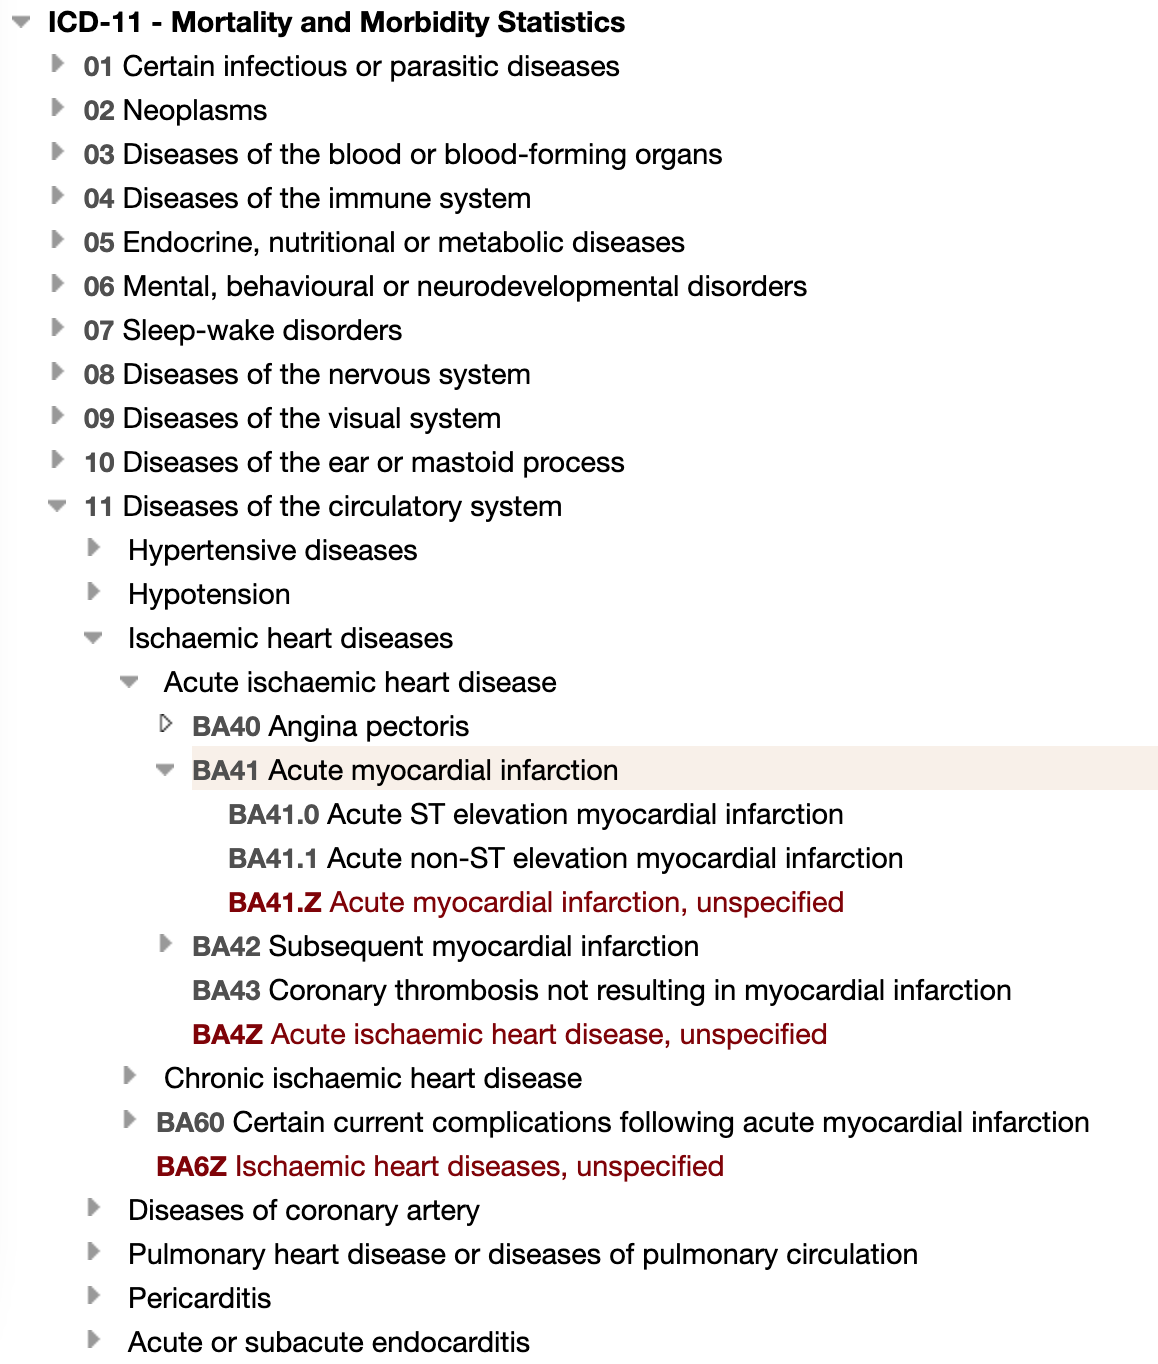
\includegraphics[width=0.8\textwidth]{icu_icd_mi}
    \caption{ICD Codes}
    \vspace{12px}
    The International Classification of Diseases (ICD) is a taxonomy of all medical conditions maintained by the World Health Organization.  "Acute myocardial infarction", for example, is a descendant of "Acute ischemic heart diseases", which itself is a descendant of "Ischemic heart diseases", which itself is a descendant of "Diseases of the circulatory system".  "Acute myocardial infarction" is then further subdivided if more granularity is required.
    \label{fig:icu_icd_mi}
    \end{figure}
}

\def \figIcuExampleWaveforms {
    \begin{figure}
    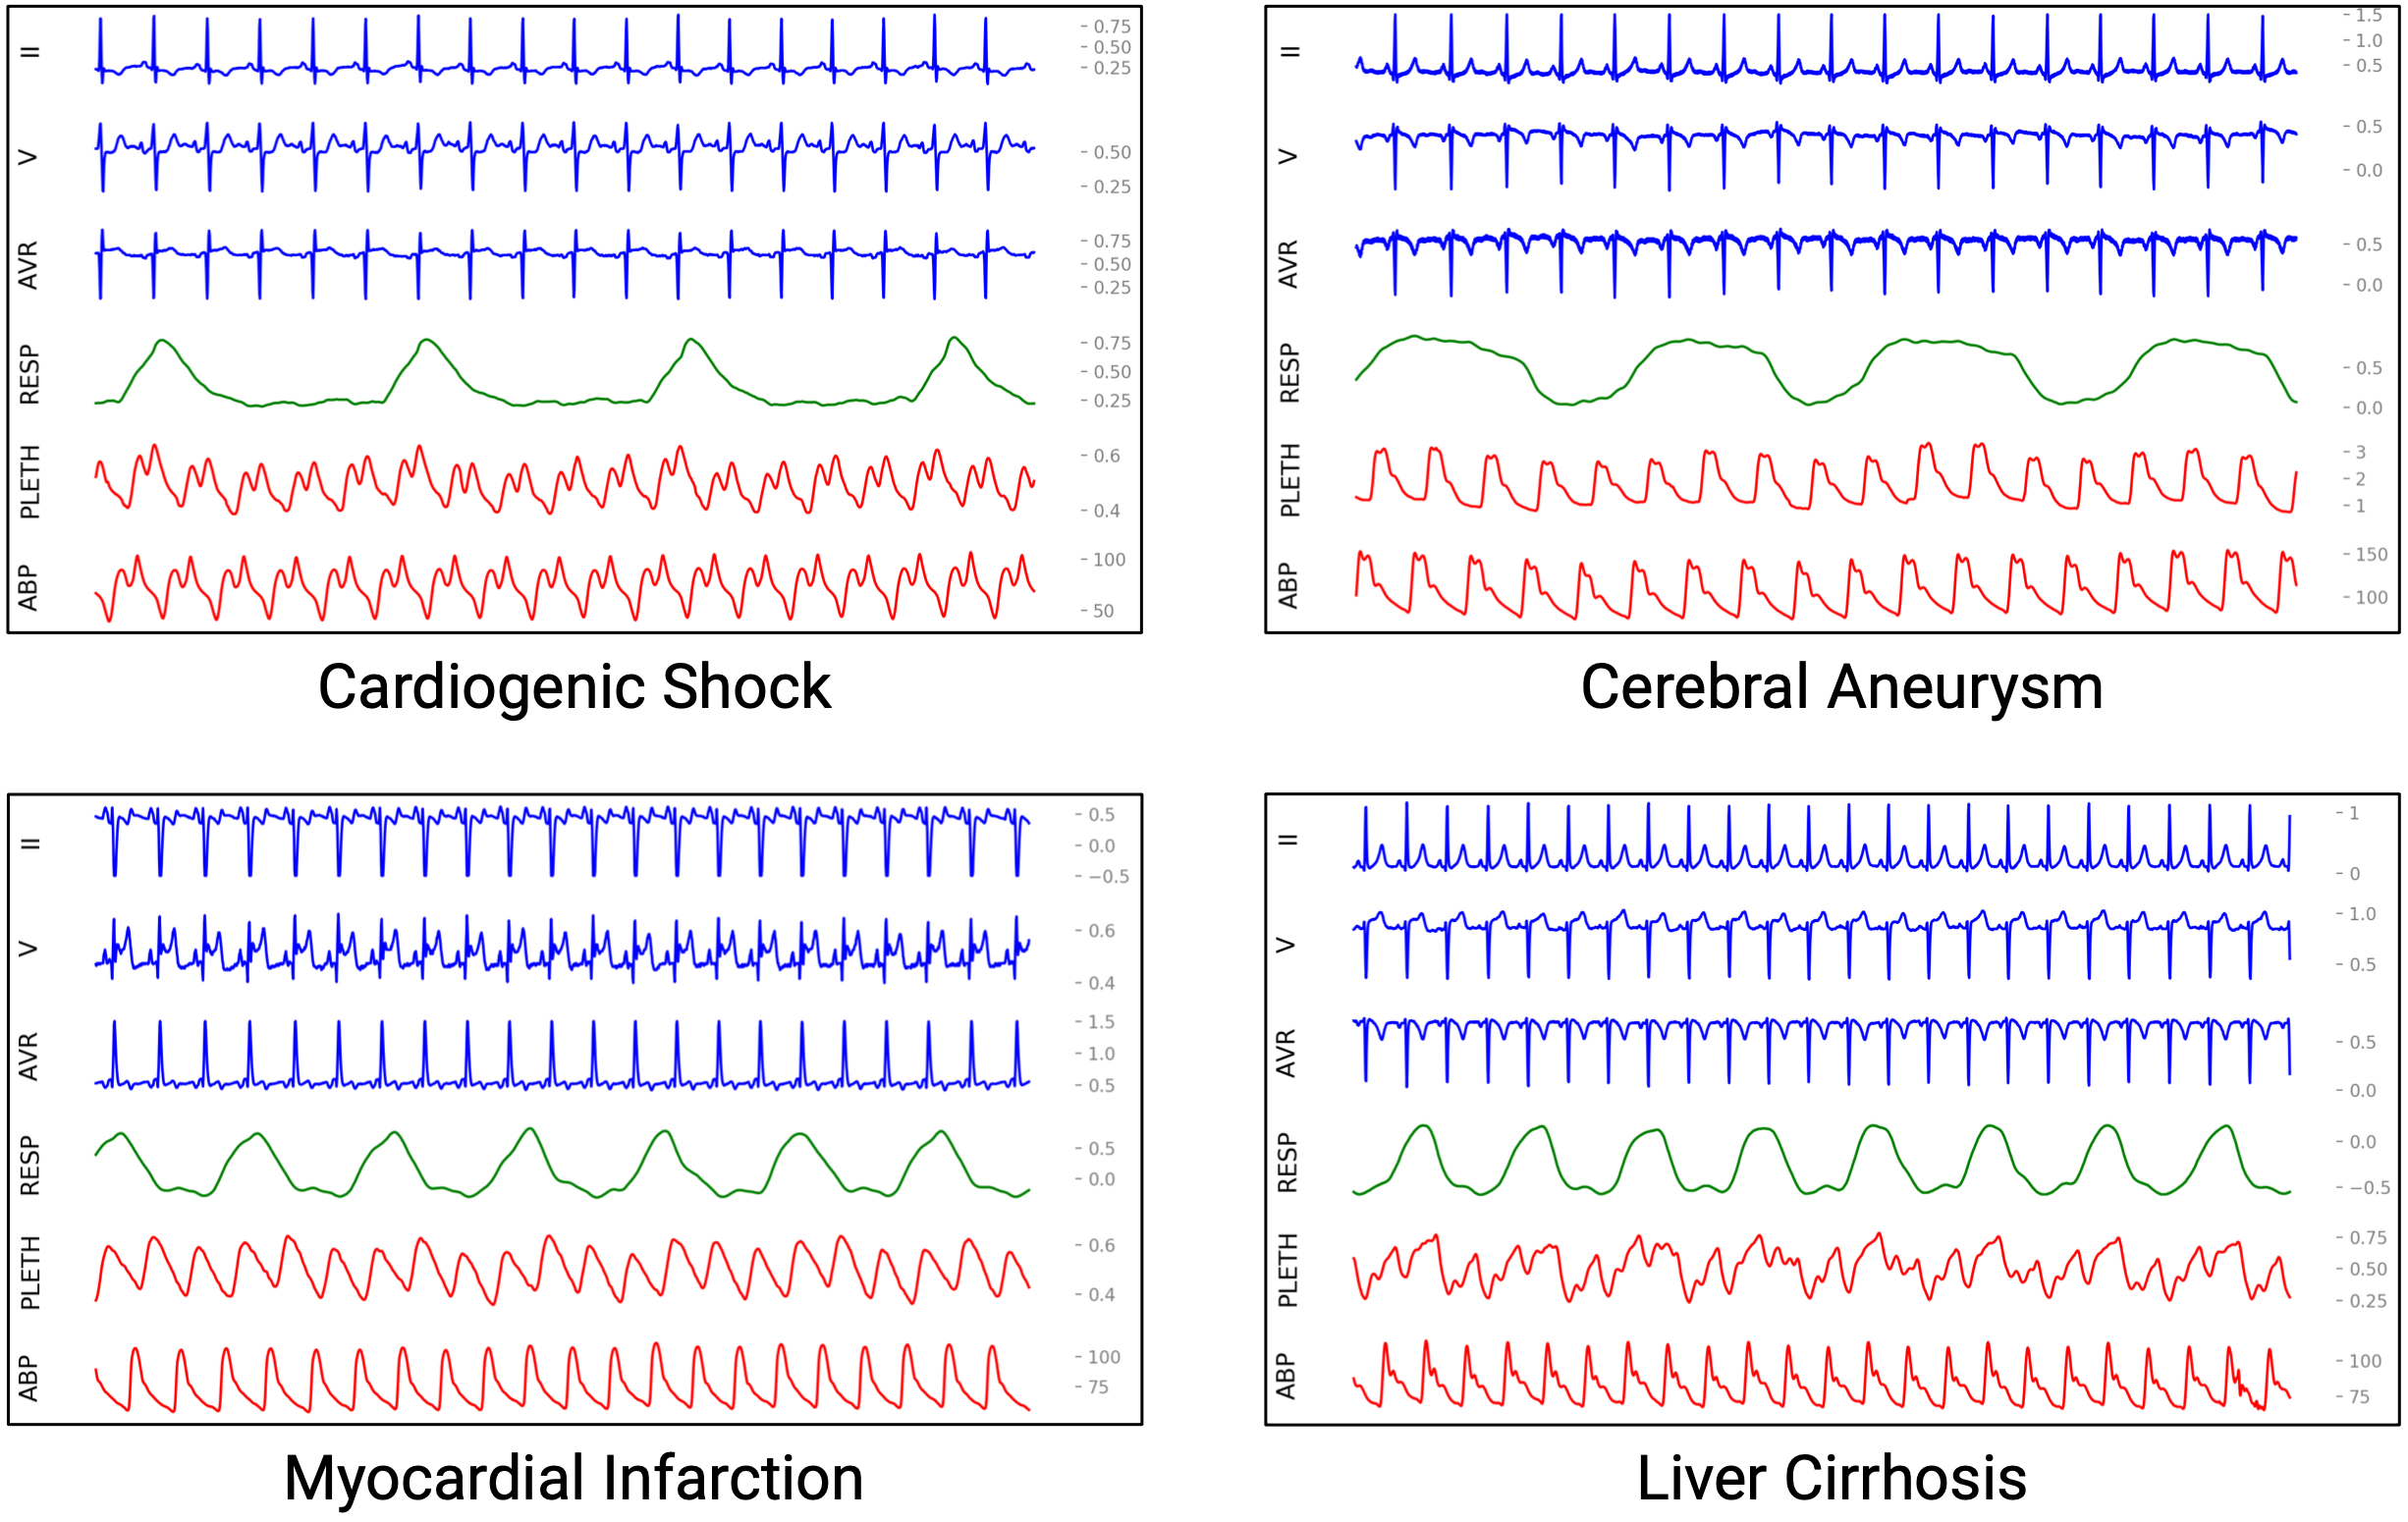
\includegraphics[width=\textwidth]{icu_example_inputs}
    \caption{Example inputs}
    \vspace{12px}
    Waveforms are sampled at 125Hz with 8 bit resolution.  An example contains 2048 samples, or about 16 seconds.  Waveform types include 3 ECG leads (II, V, AVR) shown in blue, respiration shown in in green, and photoplethysmogram and arterial blood pressure, both shown in red.  An example is labeled with a set of ICD codes.  The examples shown were correctly detected by the net.  That is, the patient that produced the waveforms shown was eventually diagnosed with the ICD code below.  In the upper left we see an example from a patient that was correctly flagged for cardiogenic shock.  The the upper right we have an example of a detected cerebral aneurysm.  In the lower left and right we have examples of myocardial infarction and liver cirrhosis.
    \label{fig:icu_example_waveforms}
    \end{figure}
}

% \def \figIcuModelArch {
%     \begin{figure}
%     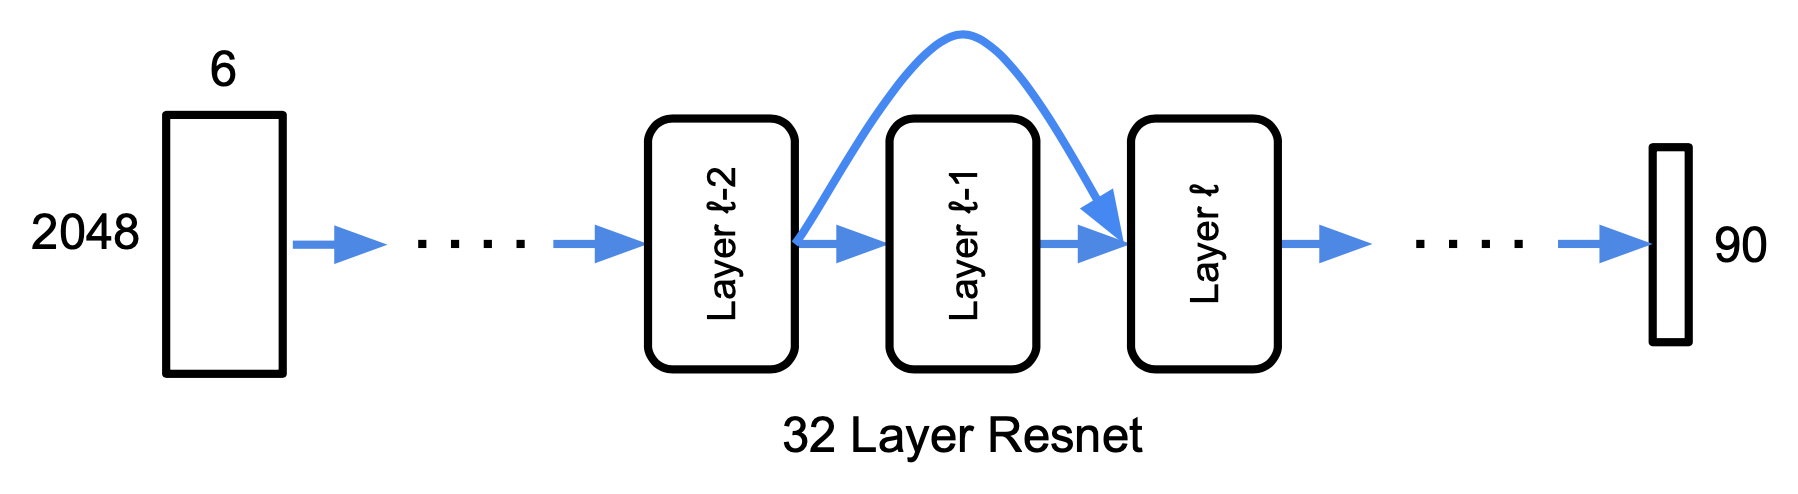
\includegraphics[width=\textwidth]{icu_model_arch}
%     \caption{Model architecture}
%     \vspace{12px}
%     A 32 layer 1D ConvNet with residual layers was trained on inputs of $k$ by 2048.  During training time, $k = 15$, and during inference time $k = 6$.  The discrepancy in $k$ is due to the fact that not all waveforms are present for every patient.  The patients in the validation and test sets are restricted to those who have all 6 of the required waveforms measured.  During training, missing waveforms are input as 0 vectors.  The net outputs 90 probabilities, 1 for each of the 90 ICD codes trained on.  Each example can have multiple diagnoses associated with it.  The loss is the mean of all 90 binary cross entropies.
%     \label{fig:icu_model_arch}
%     \end{figure}
% }

\def \figIcuCardio {
    \begin{figure}
    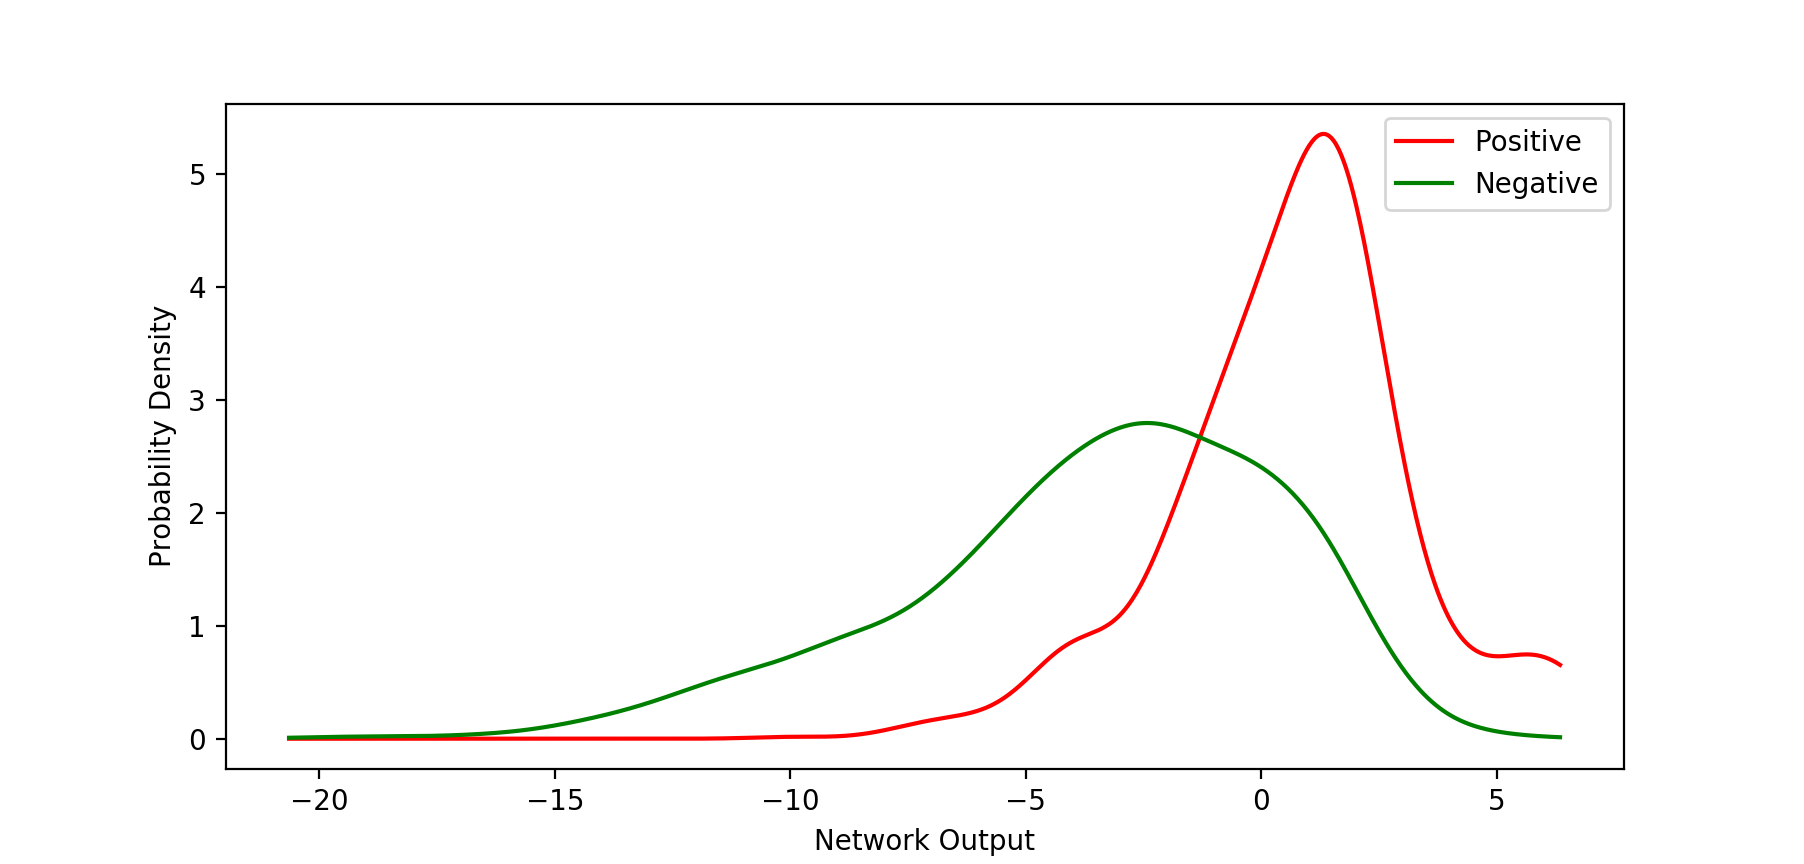
\includegraphics[width=\textwidth]{icu_cardio_prob}
    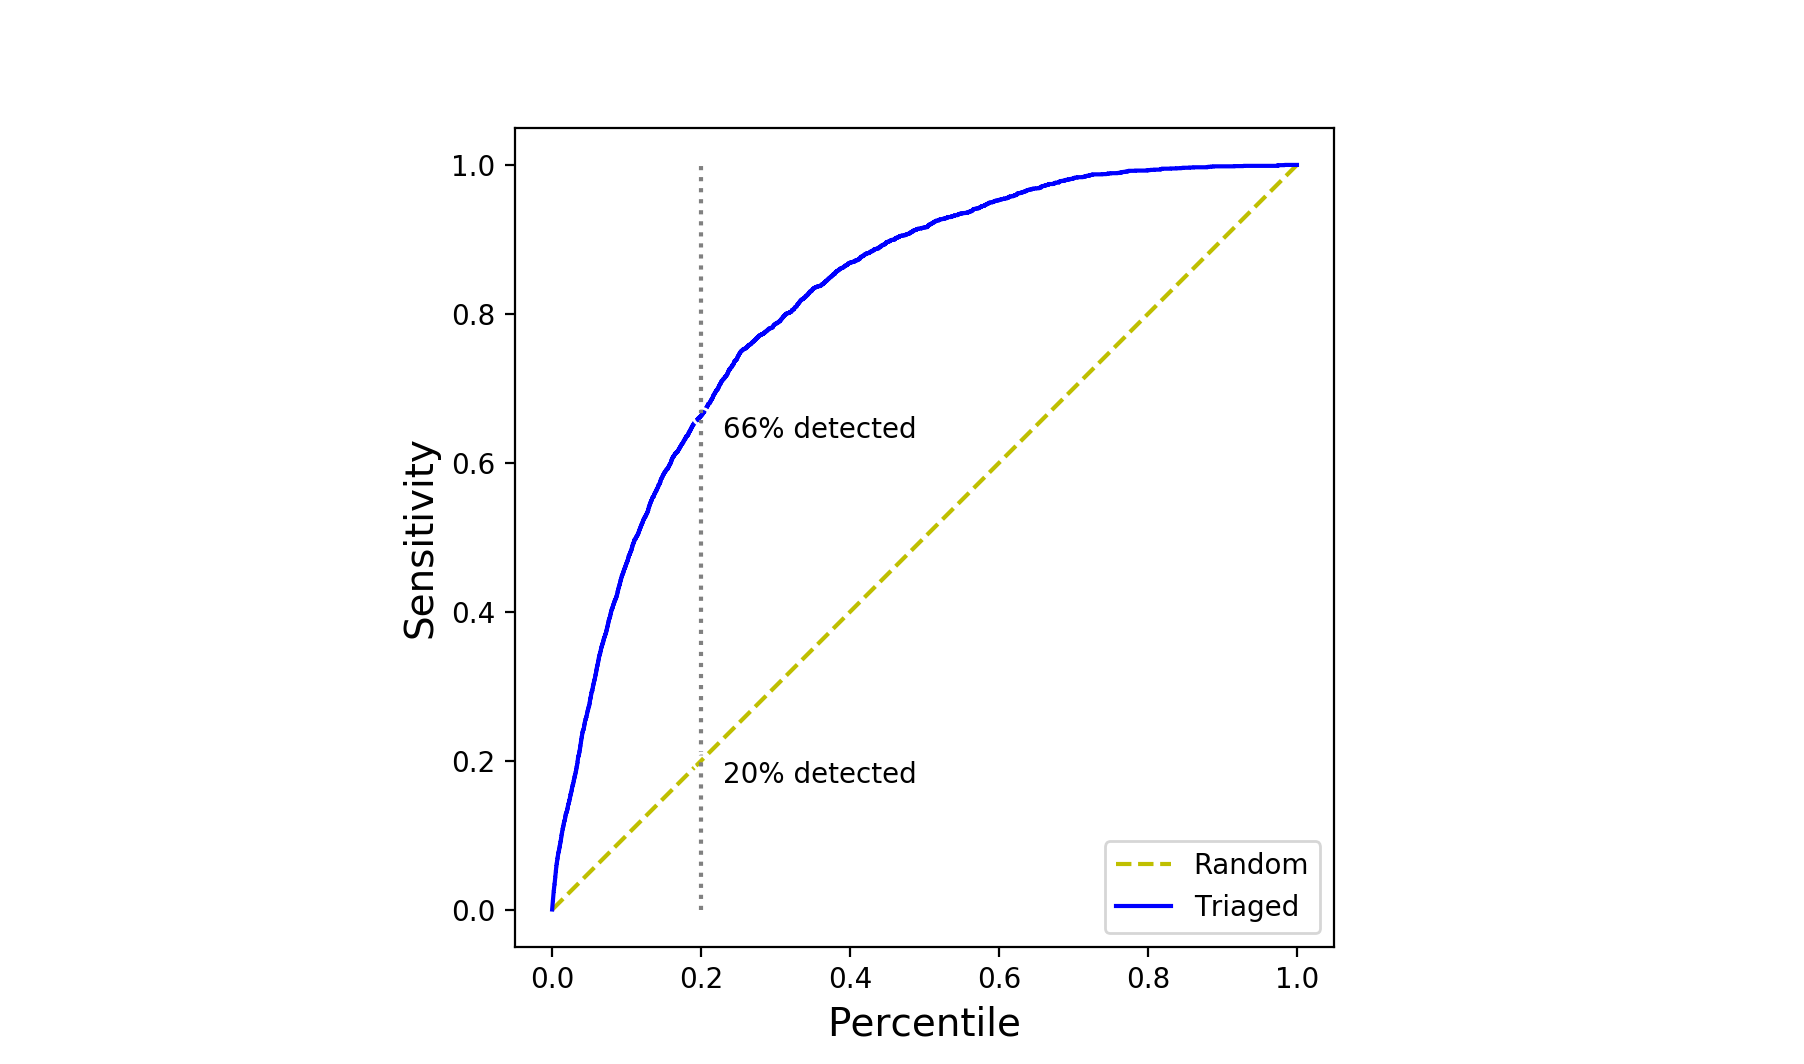
\includegraphics[width=\textwidth]{icu_cardio_sens}
    \caption{Cardiogenic Shock Results}
    \vspace{12px}
    (a) Kernel density estimates of the net's output given whether the patient eventually receives a positive or negative diagnosis for cardiogenic shock. (b) Effective sensitivity of the network for detecting a cardiogenic shock.  Using the net to flag the 20 percentile patients at highest risk for further testing would detect 66\% of the cases.
    \label{fig:icu_cardio}
    \end{figure}
}

\def \figIcuSystolic {
    \begin{figure}
    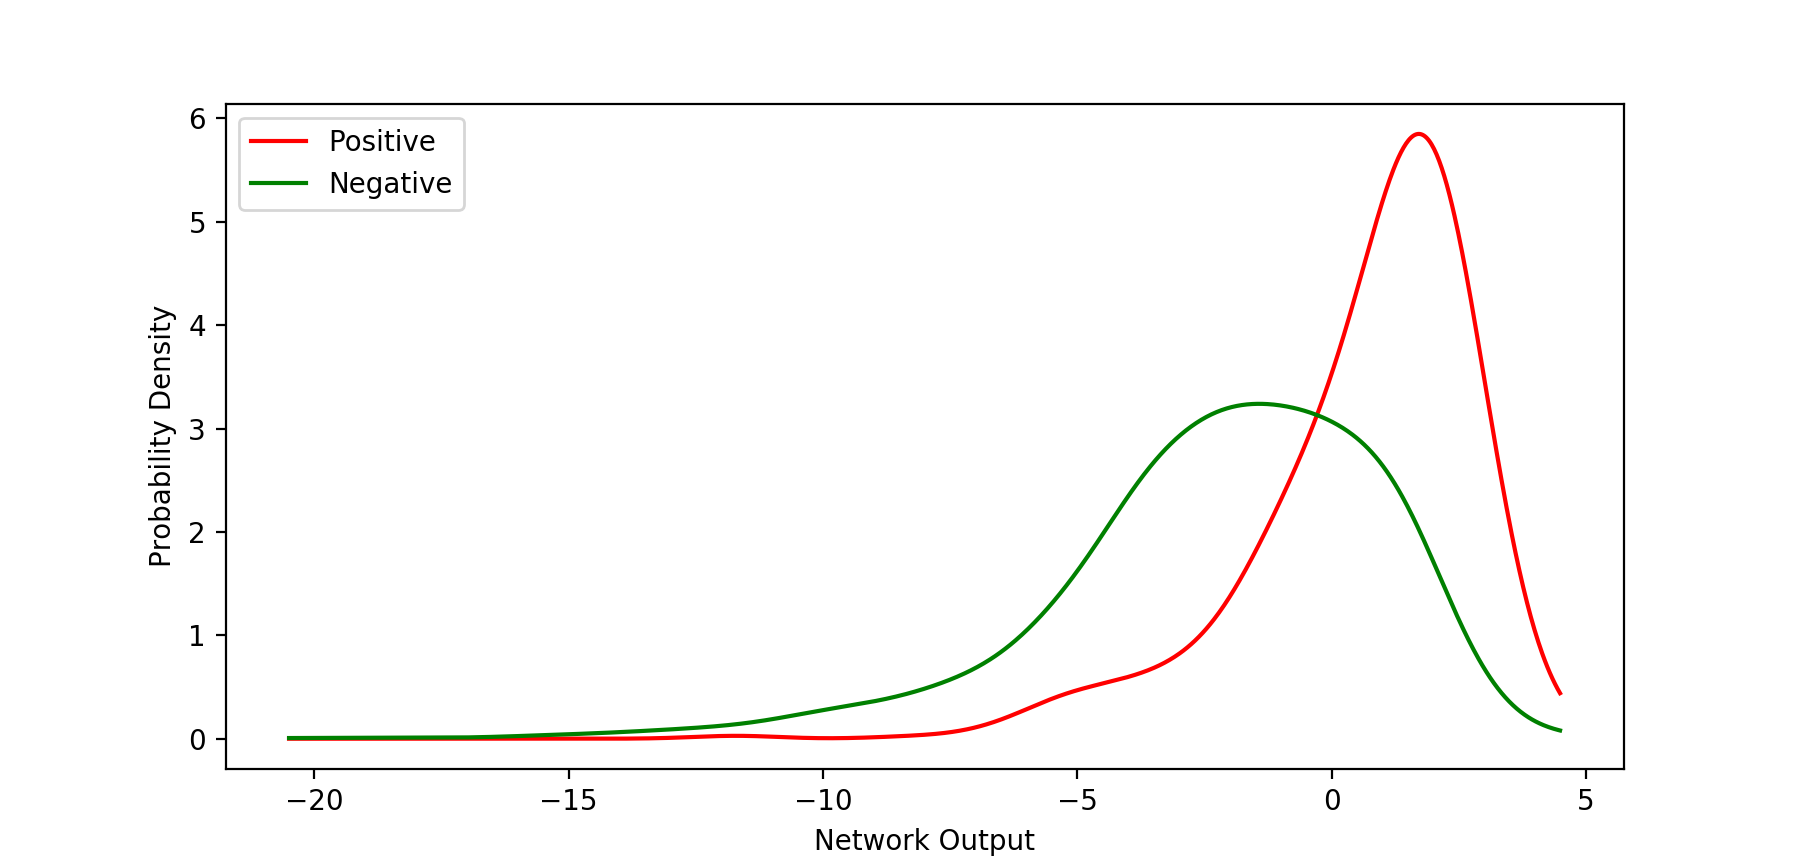
\includegraphics[width=\textwidth]{icu_systolic_prob}
    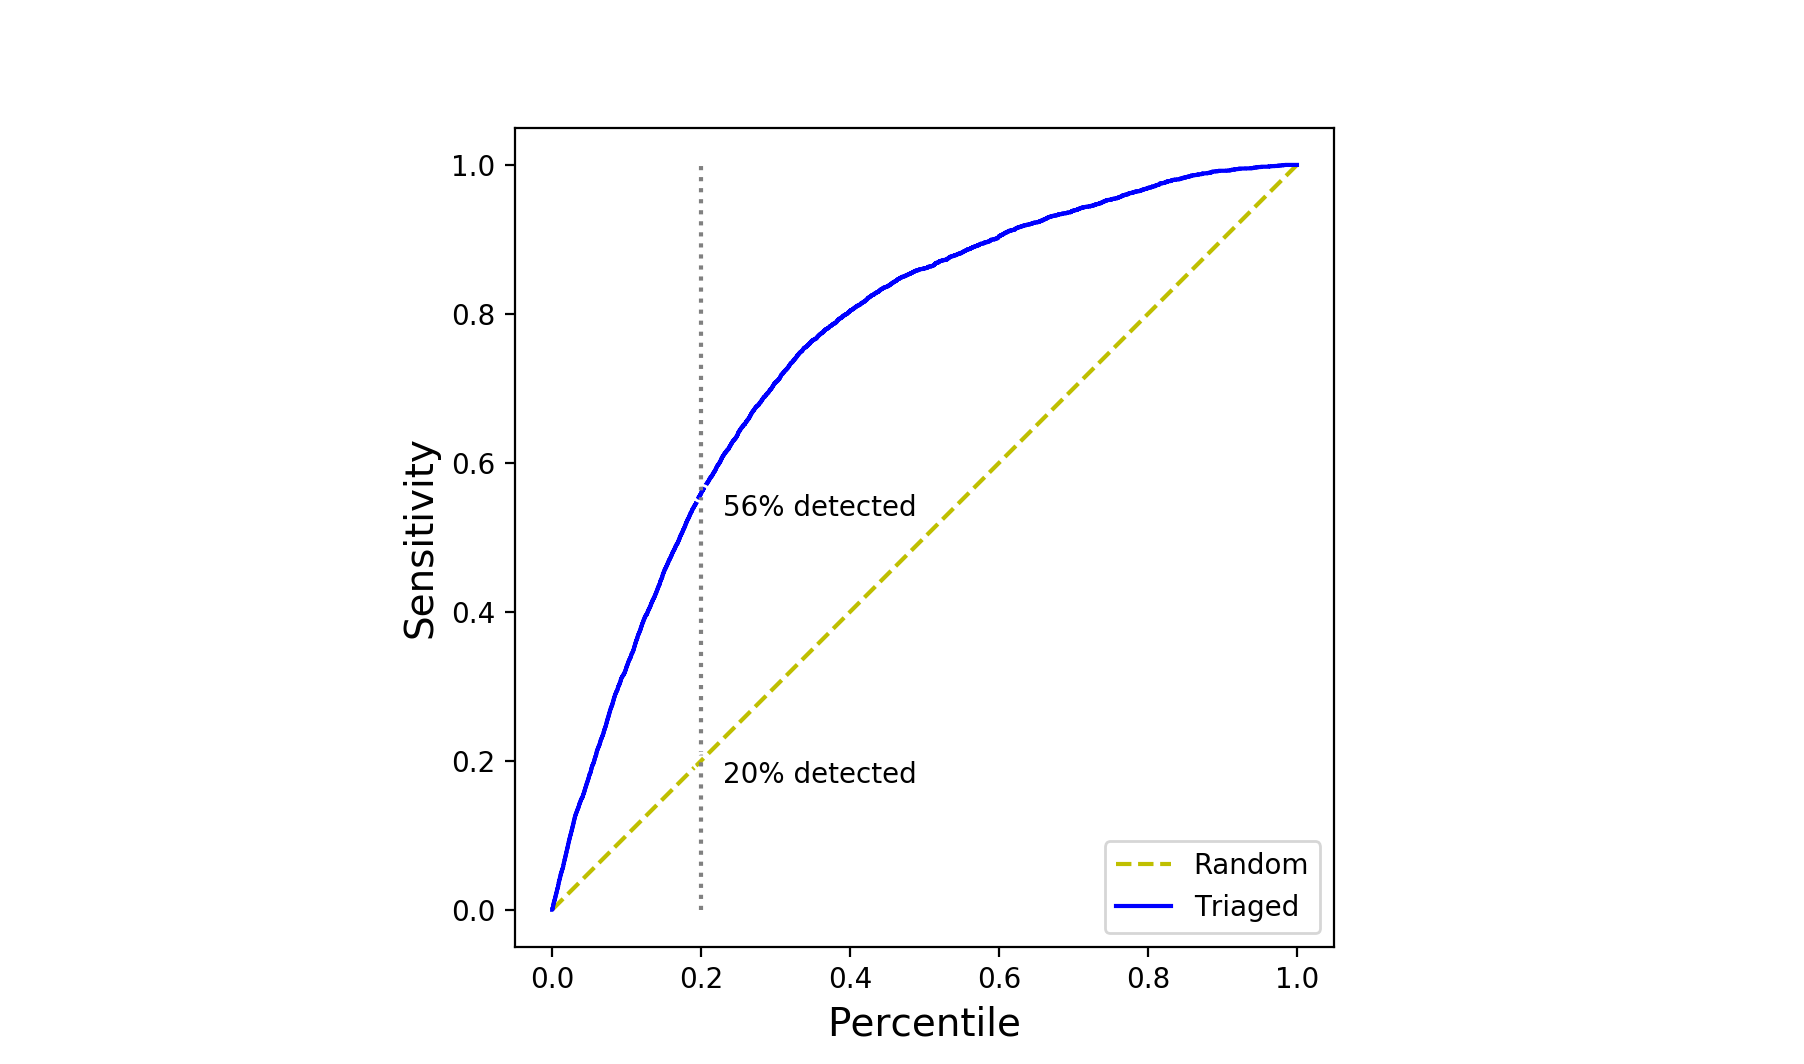
\includegraphics[width=\textwidth]{icu_systolic_sens}
    \caption{Systolic Heart Failure Results}
    \vspace{12px}
    (a) Kernel density estimates of the net's output given whether the patient eventually receives a positive or negative diagnosis for systolic heart failure. (b) Effective sensitivity of the network for detecting systolic heart failure.  Using the net to flag the 20 percentile patients at highest risk for further testing would detect 56\% of the cases.
    \label{fig:icu_systolic}
    \end{figure}
}


\def \figIcuCerebral {
    \begin{figure}
    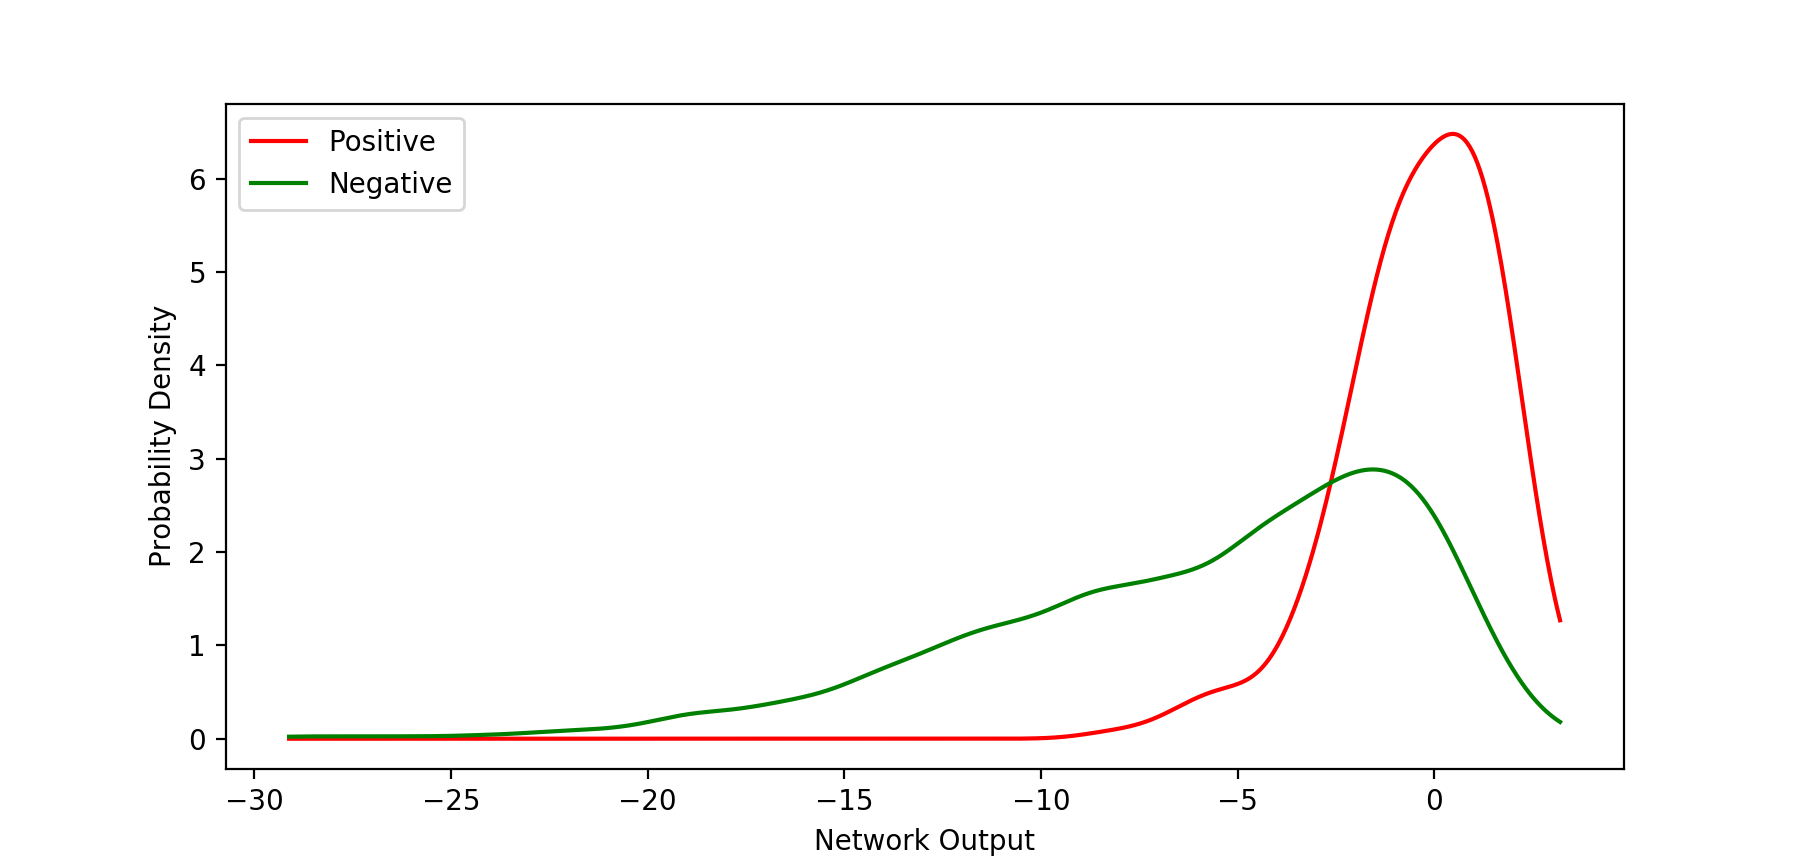
\includegraphics[width=\textwidth]{icu_cerebral_prob}
    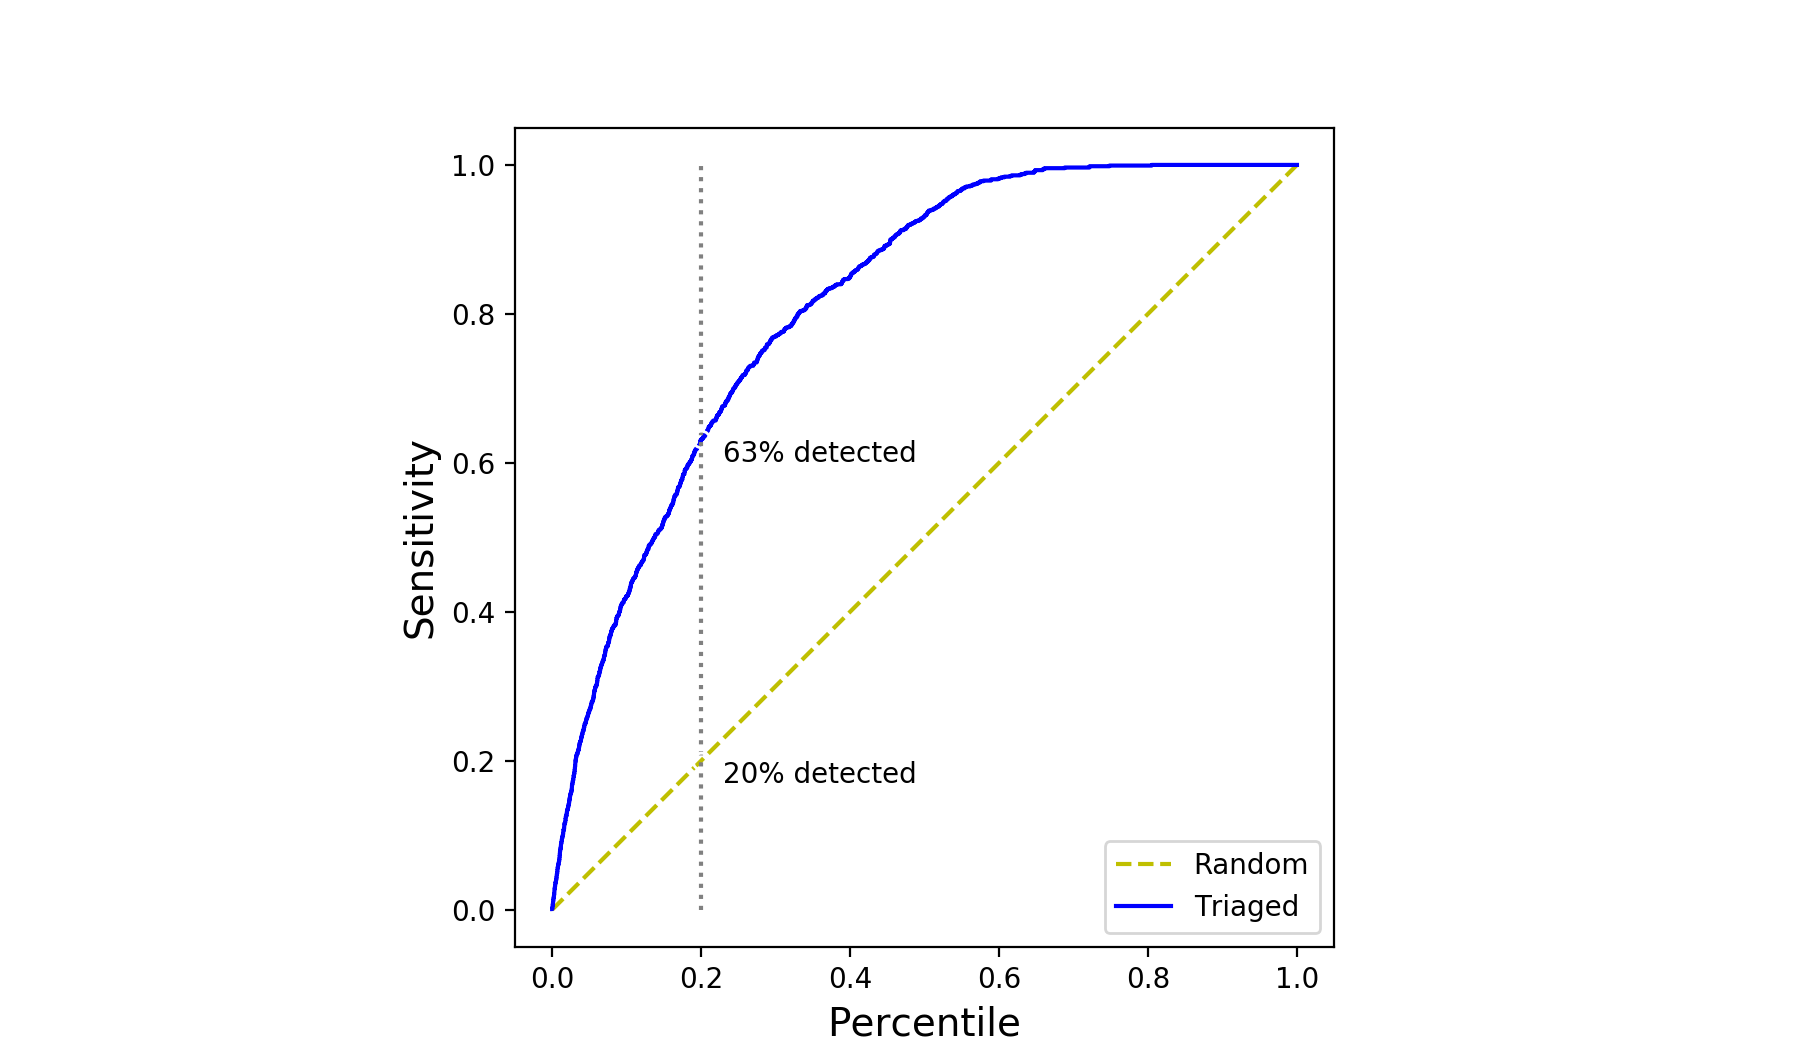
\includegraphics[width=\textwidth]{icu_cerebral_sens}
    \caption{Cerebral Aneurysm Results}
    \vspace{12px}
    (a) Kernel density estimates of the net's output given whether the patient eventually receives a positive or negative diagnosis a cerebral aneurysm. (b) Effective sensitivity of the network for detecting a cerebral aneurysm.  Using the net to flag the 20 percentile patients at highest risk for further testing would detect 63\% of the cases.
    \label{fig:icu_cerebral}
    \end{figure}
}

\def \figIcuMyocard {
    \begin{figure}
    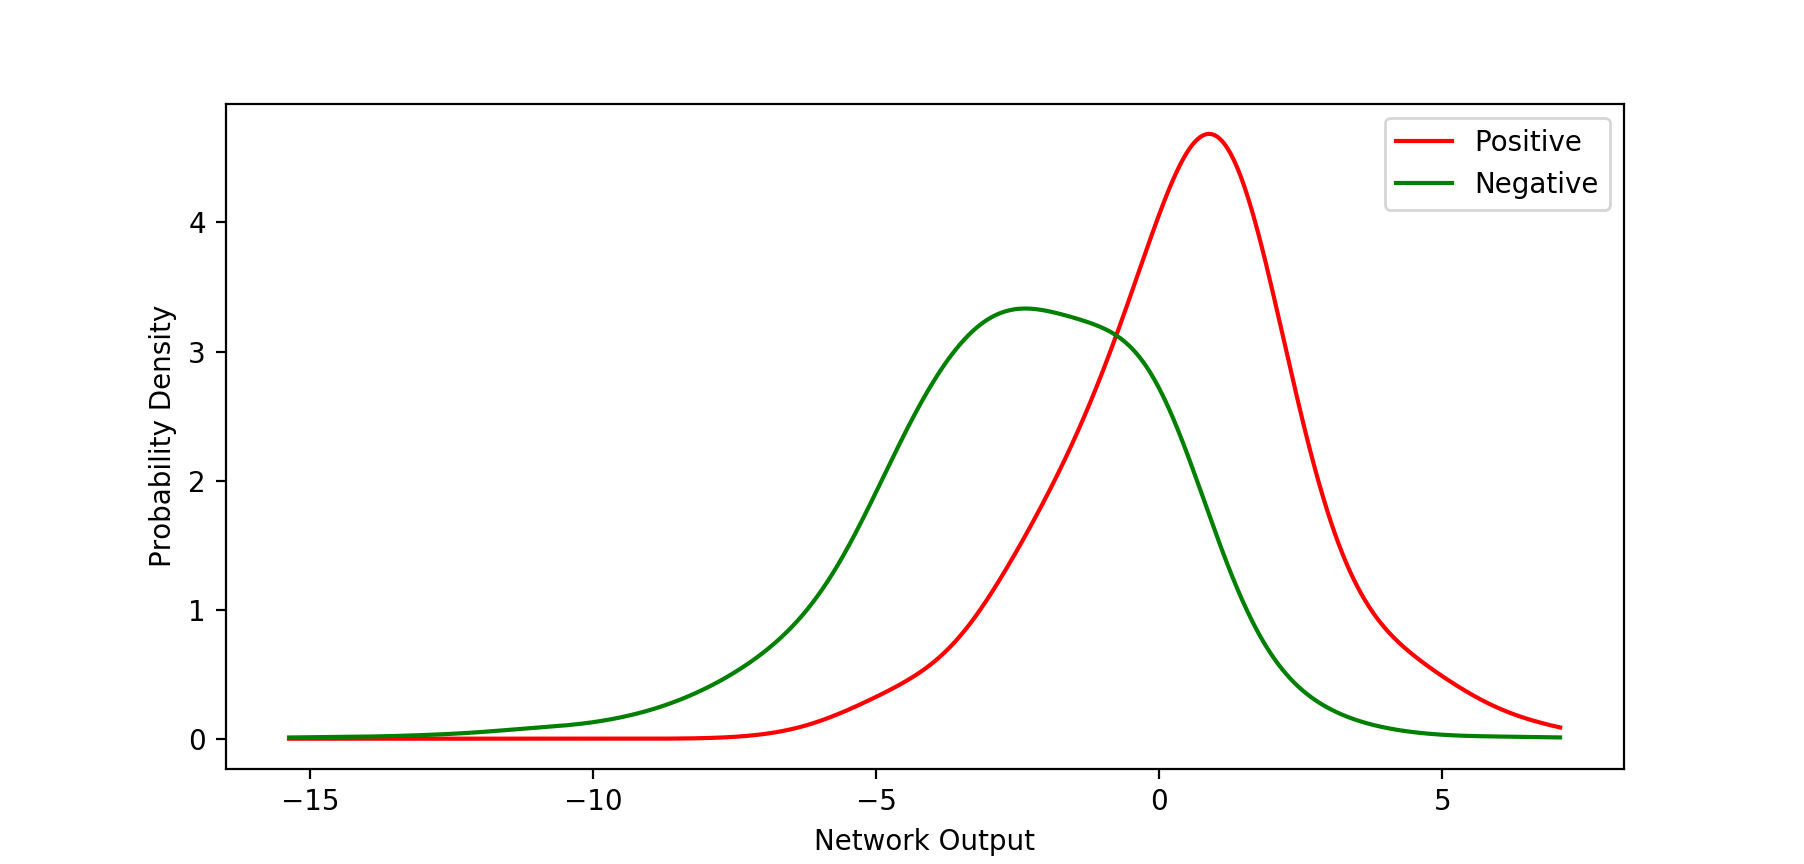
\includegraphics[width=\textwidth]{icu_myocard_prob}
    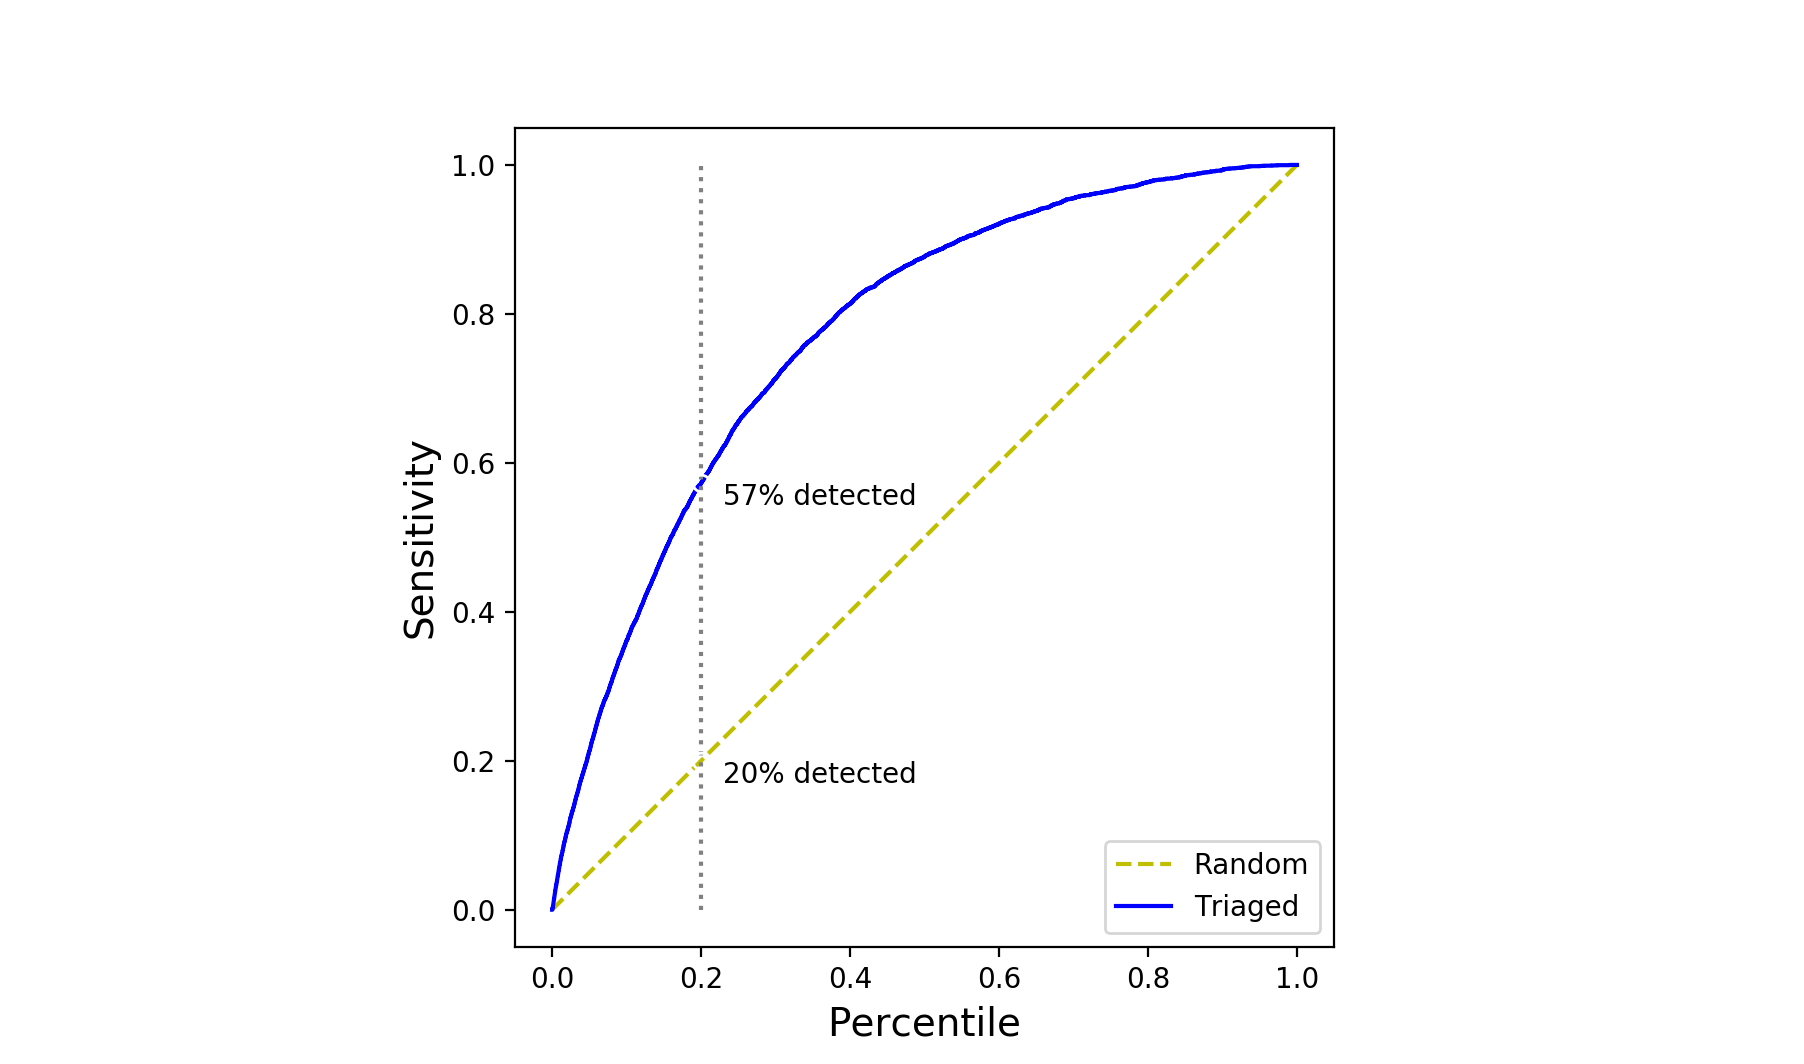
\includegraphics[width=\textwidth]{icu_myocard_sens}
    \caption{Myocardial Infarction Results}
    \vspace{12px}
    (a) Kernel density estimates of the net's output given whether the patient eventually receives a positive or negative diagnosis for myocardial infarction. (b) Effective sensitivity of the network for detecting a myocardial infarction.  Using the net to flag the 20 percentile patients at highest risk for further testing would detect 57\% of the cases.
    \label{fig:icu_myocard}
    \end{figure}
}

\def \figIcuRelativeRisk {
    \begin{figure}
    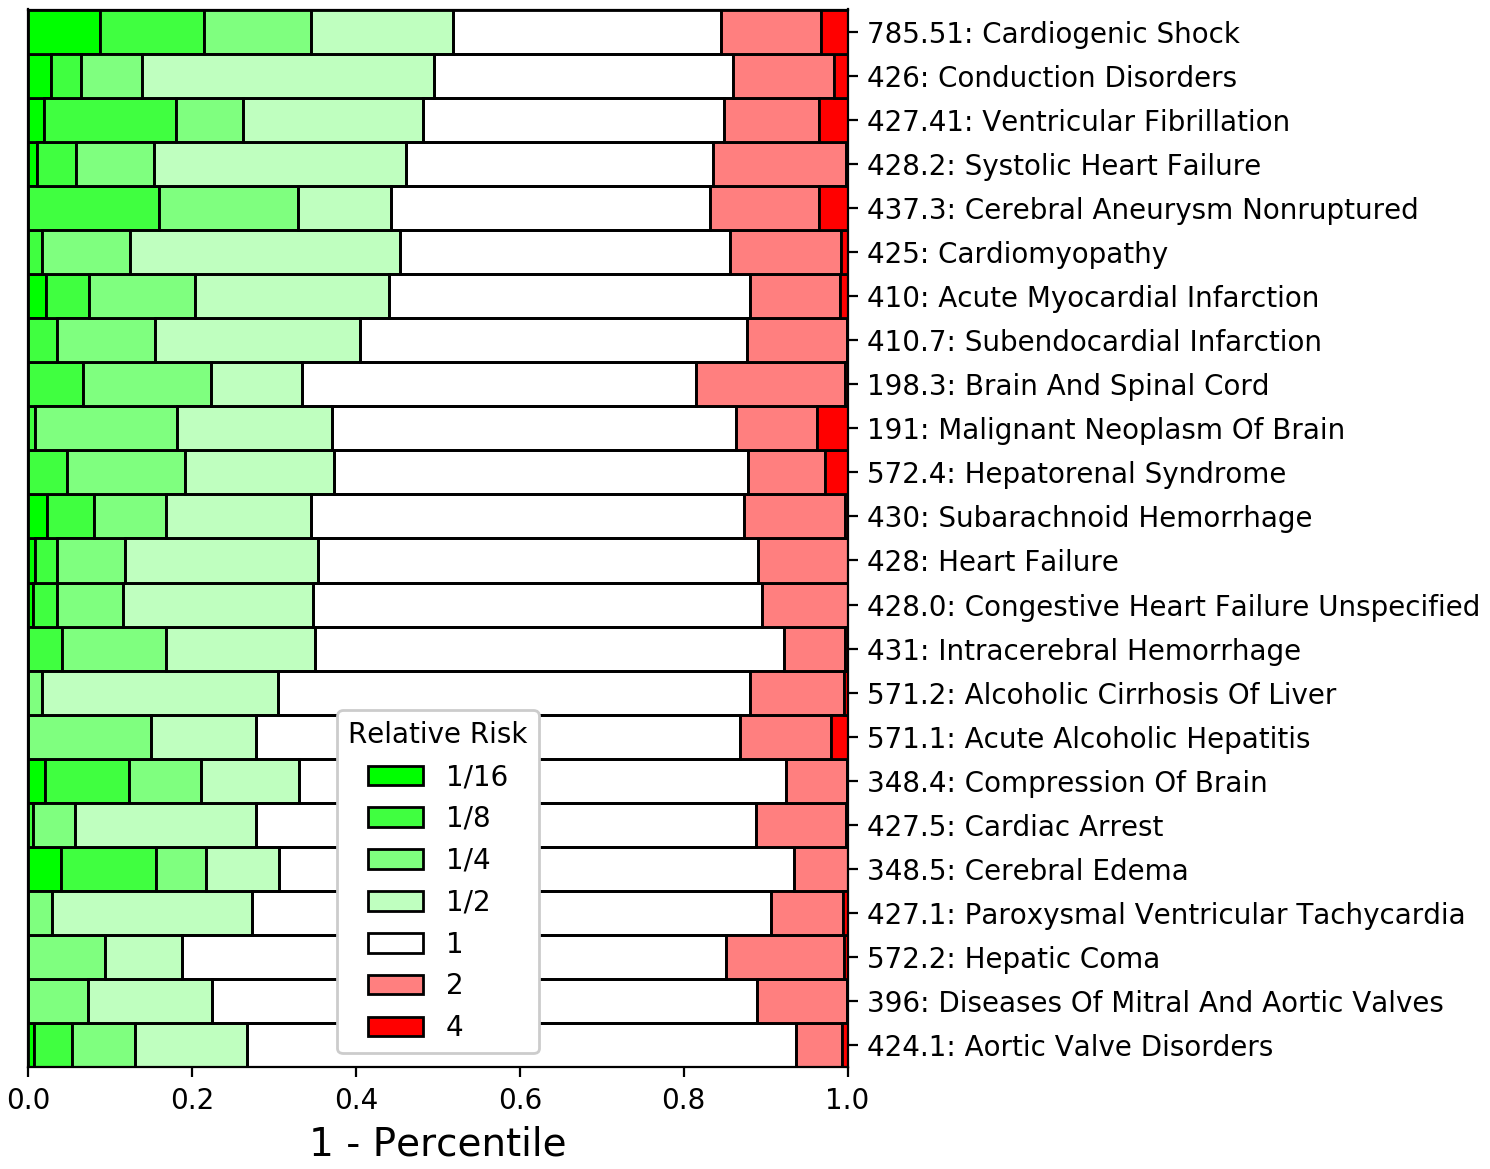
\includegraphics[width=\textwidth]{icu_relative_risk}
    \caption{Relative risk}
    \vspace{12px}
    Patients are placed into estimated risk categories of powers of 2.  For example, a patient in the 1/4 risk category of systolic heart failure is estimated to be between 1/4 and 1/8 as likely to be diagnosed with systolic heart failure.  For cardiogenic shock, about half of the patients can be placed into a low risk category.  The risk level estimates are conservative, with low risk patients actually estimated to have lower risk than the risk group they are placed in, and high risk patients estimated to have higher risk than the risk group they are placed in.
    \label{fig:icu_relative_risk}
    \end{figure}
}

\def \figIcuActualRisk {
    \begin{figure}
    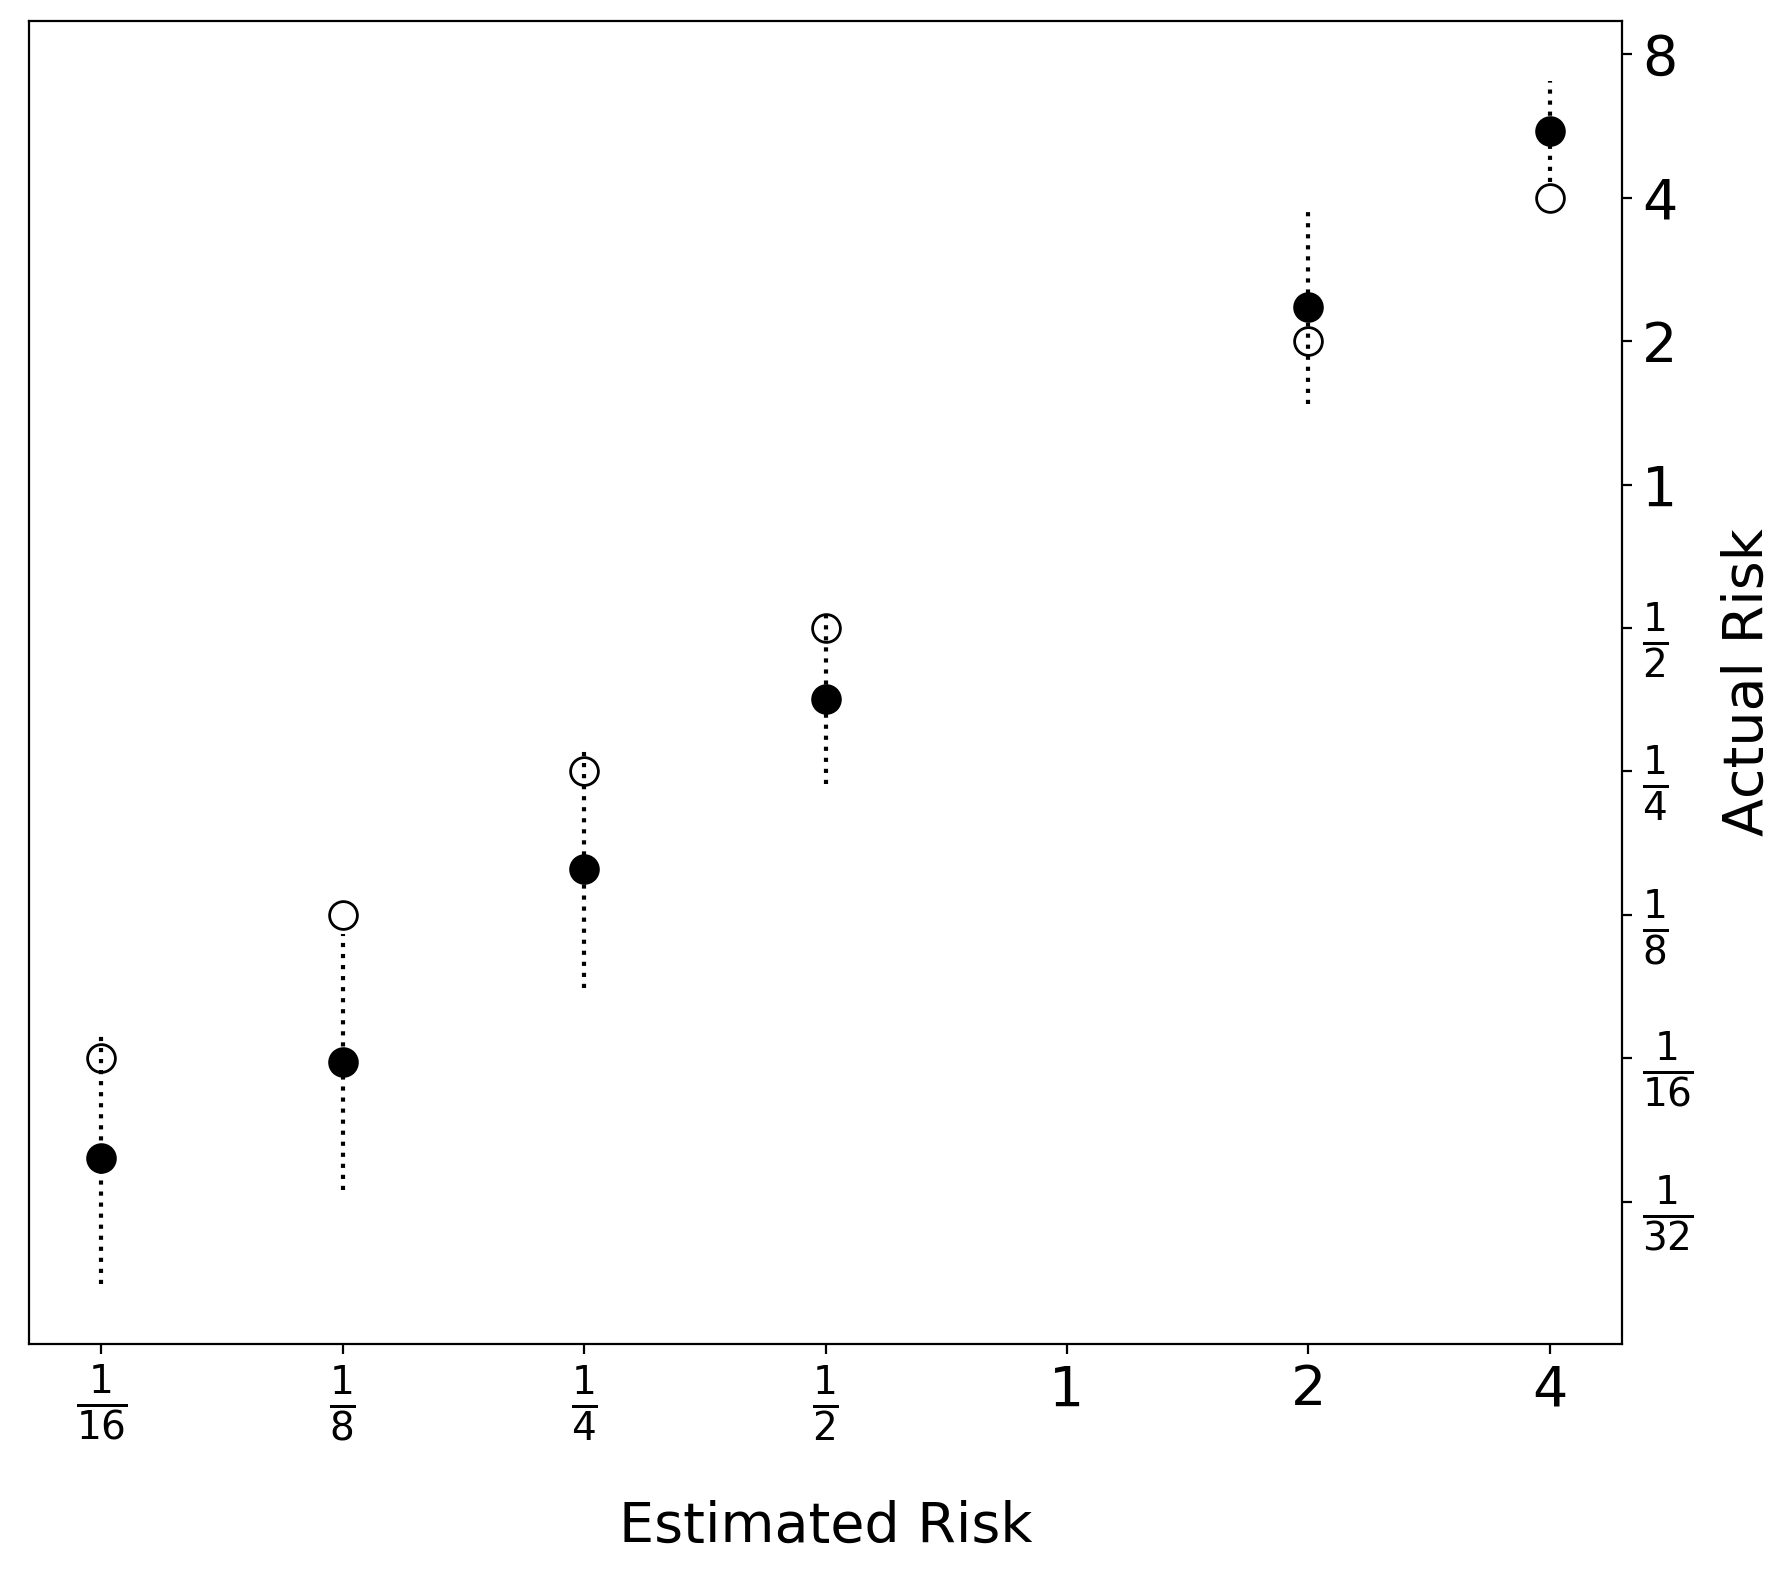
\includegraphics[width=\textwidth]{icu_actual_risk}
    \caption{Actual risk}
    \vspace{12px}
    Risk categories are valid.  For each risk category an actual risk can be computed with error bars.  The error bars represent the fact that there are 90 conditions being predicted.  Ideally the low risk categories should have an actual risk lower than the estimated risk and the high risk categories should have a risk higher than the estimated risk, since the risk estimates were conservative.
    \label{fig:icu_actual_risk}
    \end{figure}
}

\def \figIcuIcdMap {
    \begin{figure}
    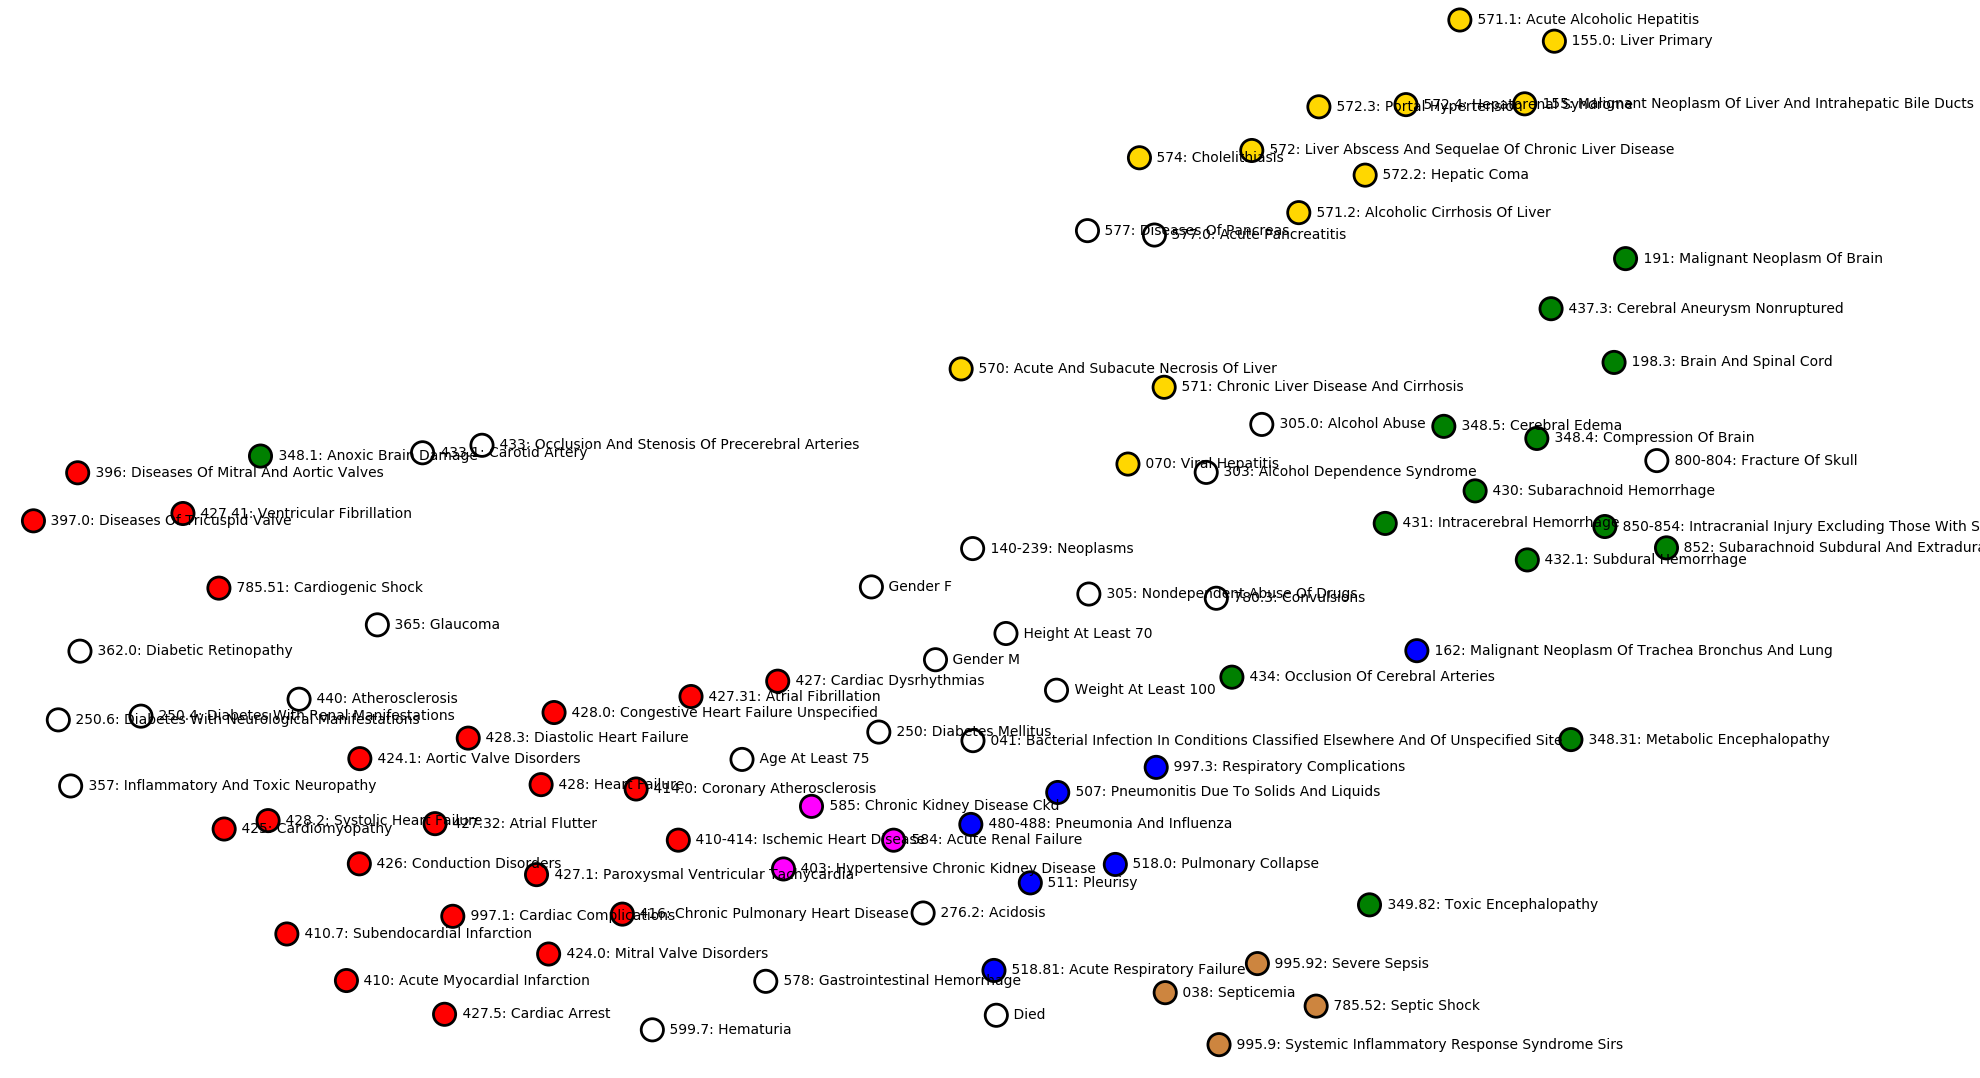
\includegraphics[width=\textwidth]{icu_icd_map}
    \caption{ICD Embedding Visualization}
    \vspace{12px}
    TSNE was applied to high dimensional ICD code embeddings to produce a 2D visualization of the ICD code space learned by the net.  Conditions affecting various organs are close together in this space.  Red circles are conditions that affect the heart.  These conditions include cardiogenic shock, coronary atherosclerosis, atrial flutter, systolic heart failure, and myocardial infarction.  Green circles are conditions that affect the brain.  These conditions include cerebral edema, brain cancer, cerebral aneurysm, intracerebral hemorrhage.  It is interesting that skull fracture found its way into this region.  Yellow circles are conditions that affect the liver.  These conditions include cirrhosis, hepatitis, and liver cancer.  It is interesting that alcohol abuse and alcohol dependence syndrome found their way into this region, and are also close to the brain conditions.  Blue circles are conditions that affect the lungs.  These conditions include pulmonary collapse, pneumonia, and acute respiratory failure.  This embedding also puts similar ICD codes together that may be far apart in the ICD taxonomy.  For example consider ICD code 785.52: Septic Shock, ICD code 995.92: Severe Sepsis, and ICD code 038: Septicemia.  The nearest common ancestor of these ICD codes in the taxonomy is the root of the entire taxonomy of all medical conditions that exist.  But the net learned that they were similar semantically based on the waveforms it was trained with.
    \label{fig:icu_icd_map}
    \end{figure}
}

\def \figIcuMaps {
    % \begin{figure}
    % 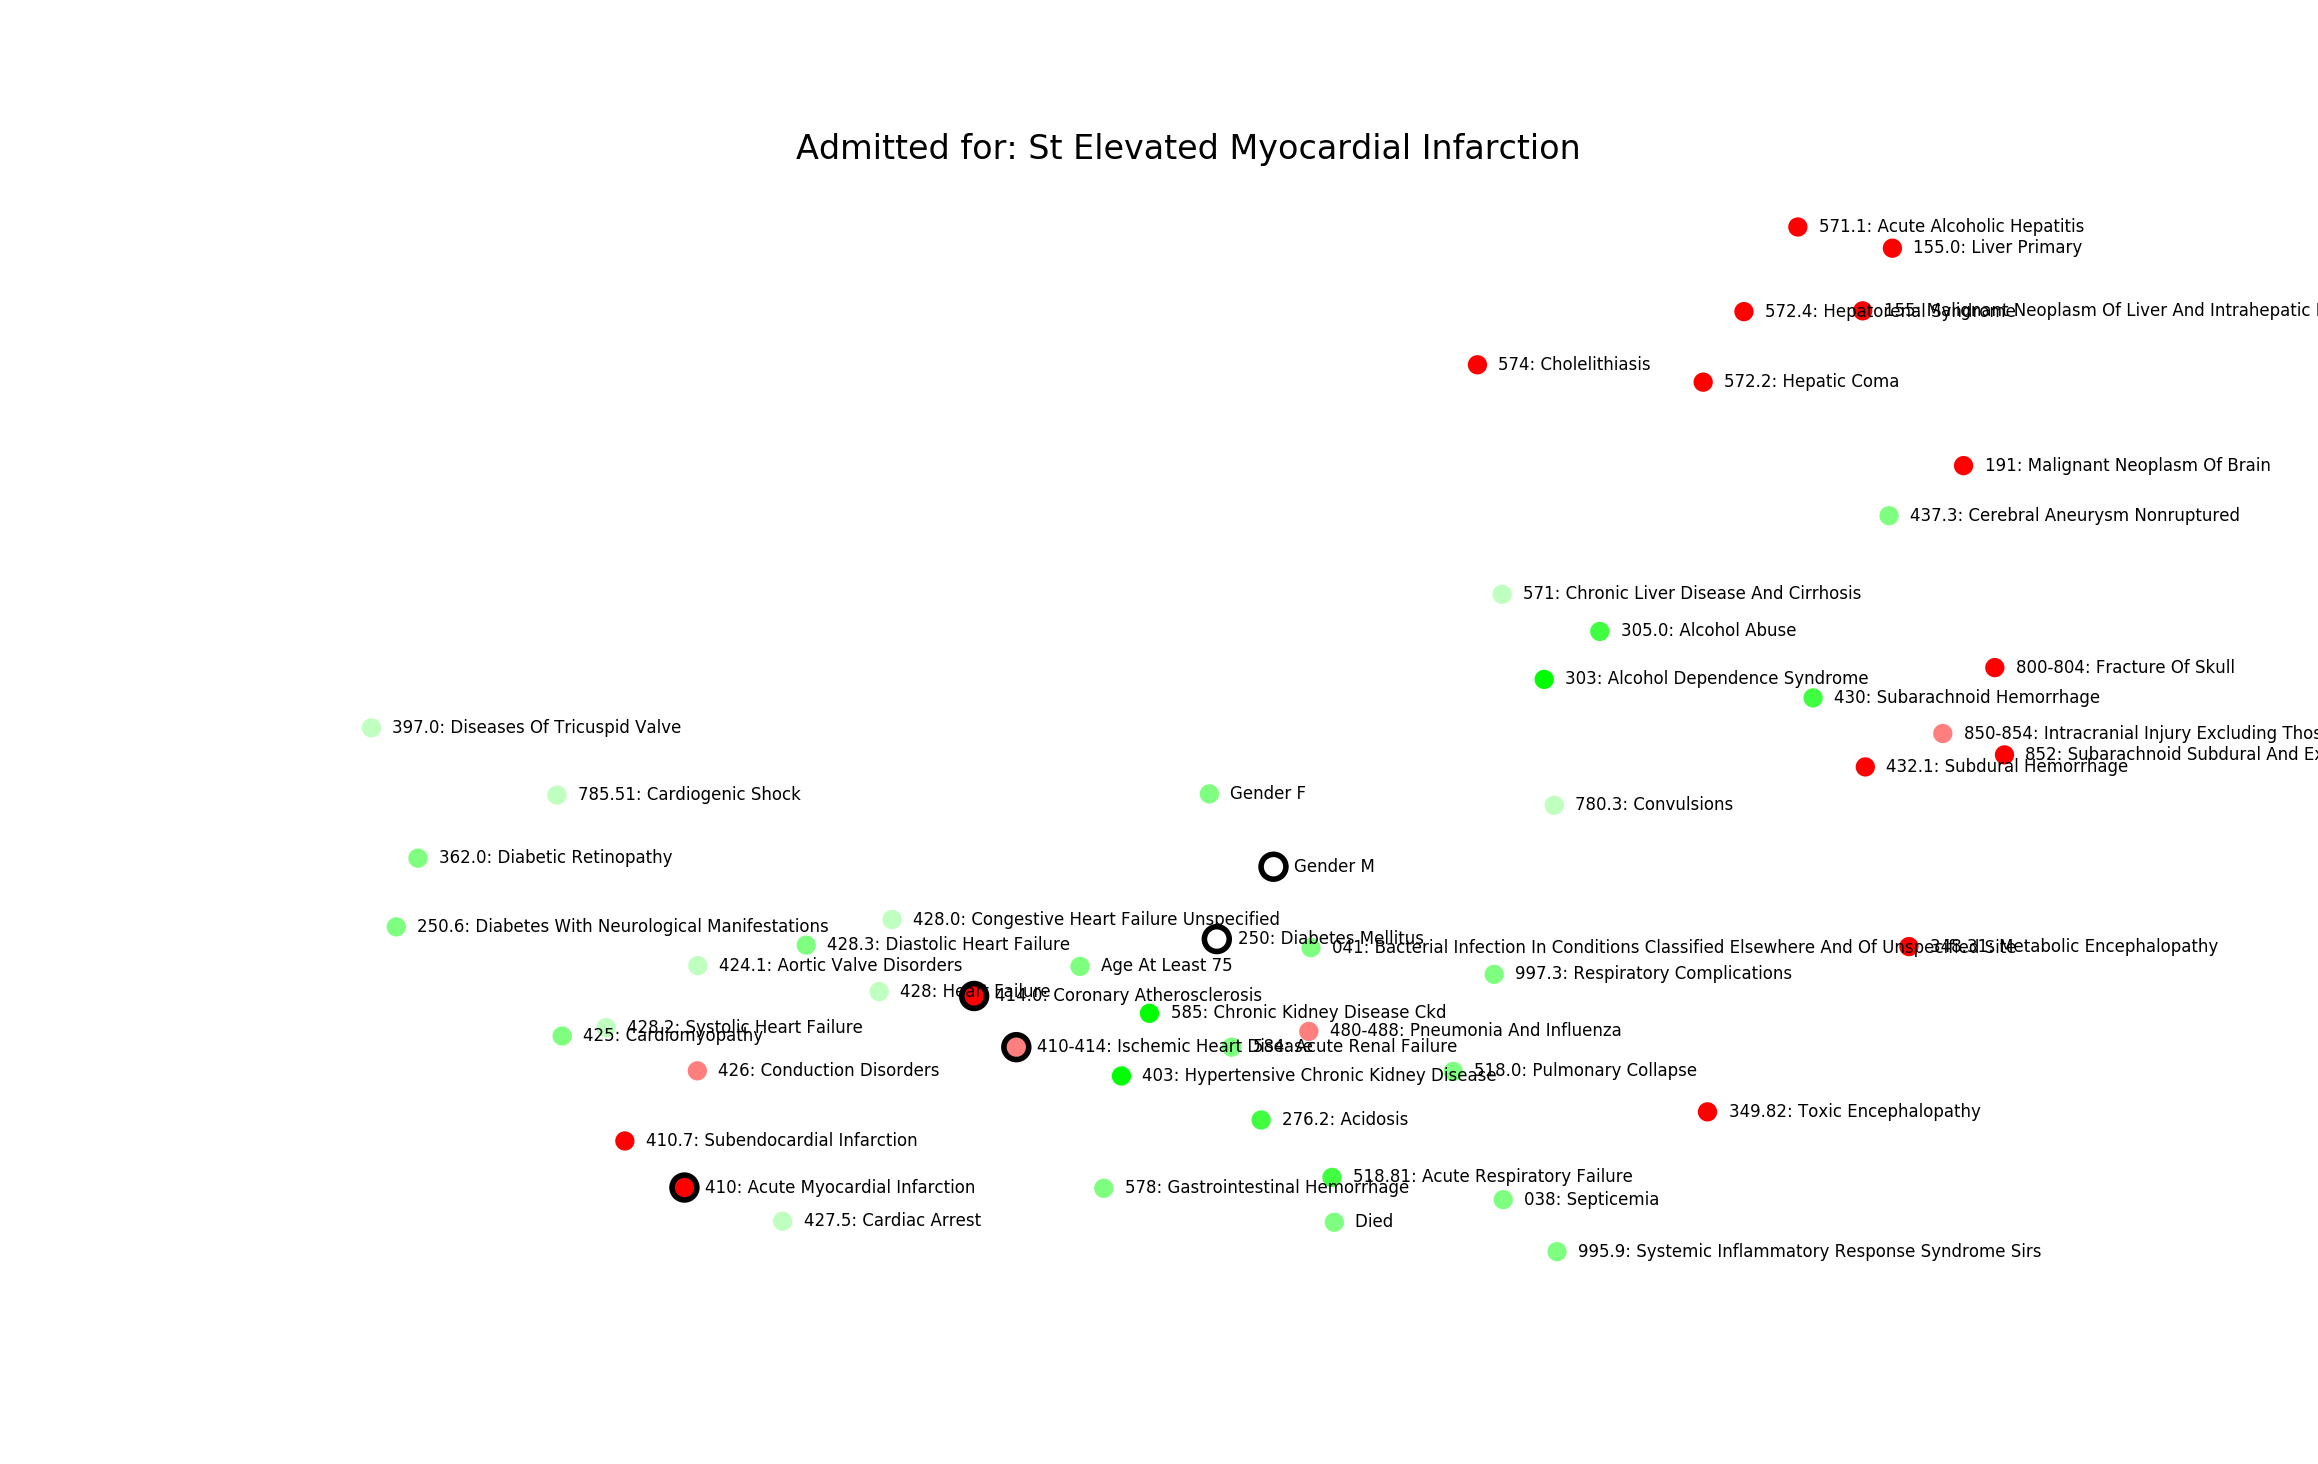
\includegraphics[width=\textwidth]{icu_map_mi}
    % \caption{Semantic Inference Myocardial Infarction}
    % \vspace{12px}
    % This patient was admitted for "ST Elevated Myocardial Infarction".  The neural net correctly predicted that they had low risk of kidney conditions, death, and many heart conditions (colored green).  It predicted high risk of liver conditions and various heart conditions including myocardial infarction and coronary atherosclerosis (colored red).  The patients was eventually in fact diagnosed with myocardial infarction and coronary atherosclerosis among other things (circled in black).
    % \label{fig:icu_map_mi}
    % \end{figure}
    
    \begin{figure}
    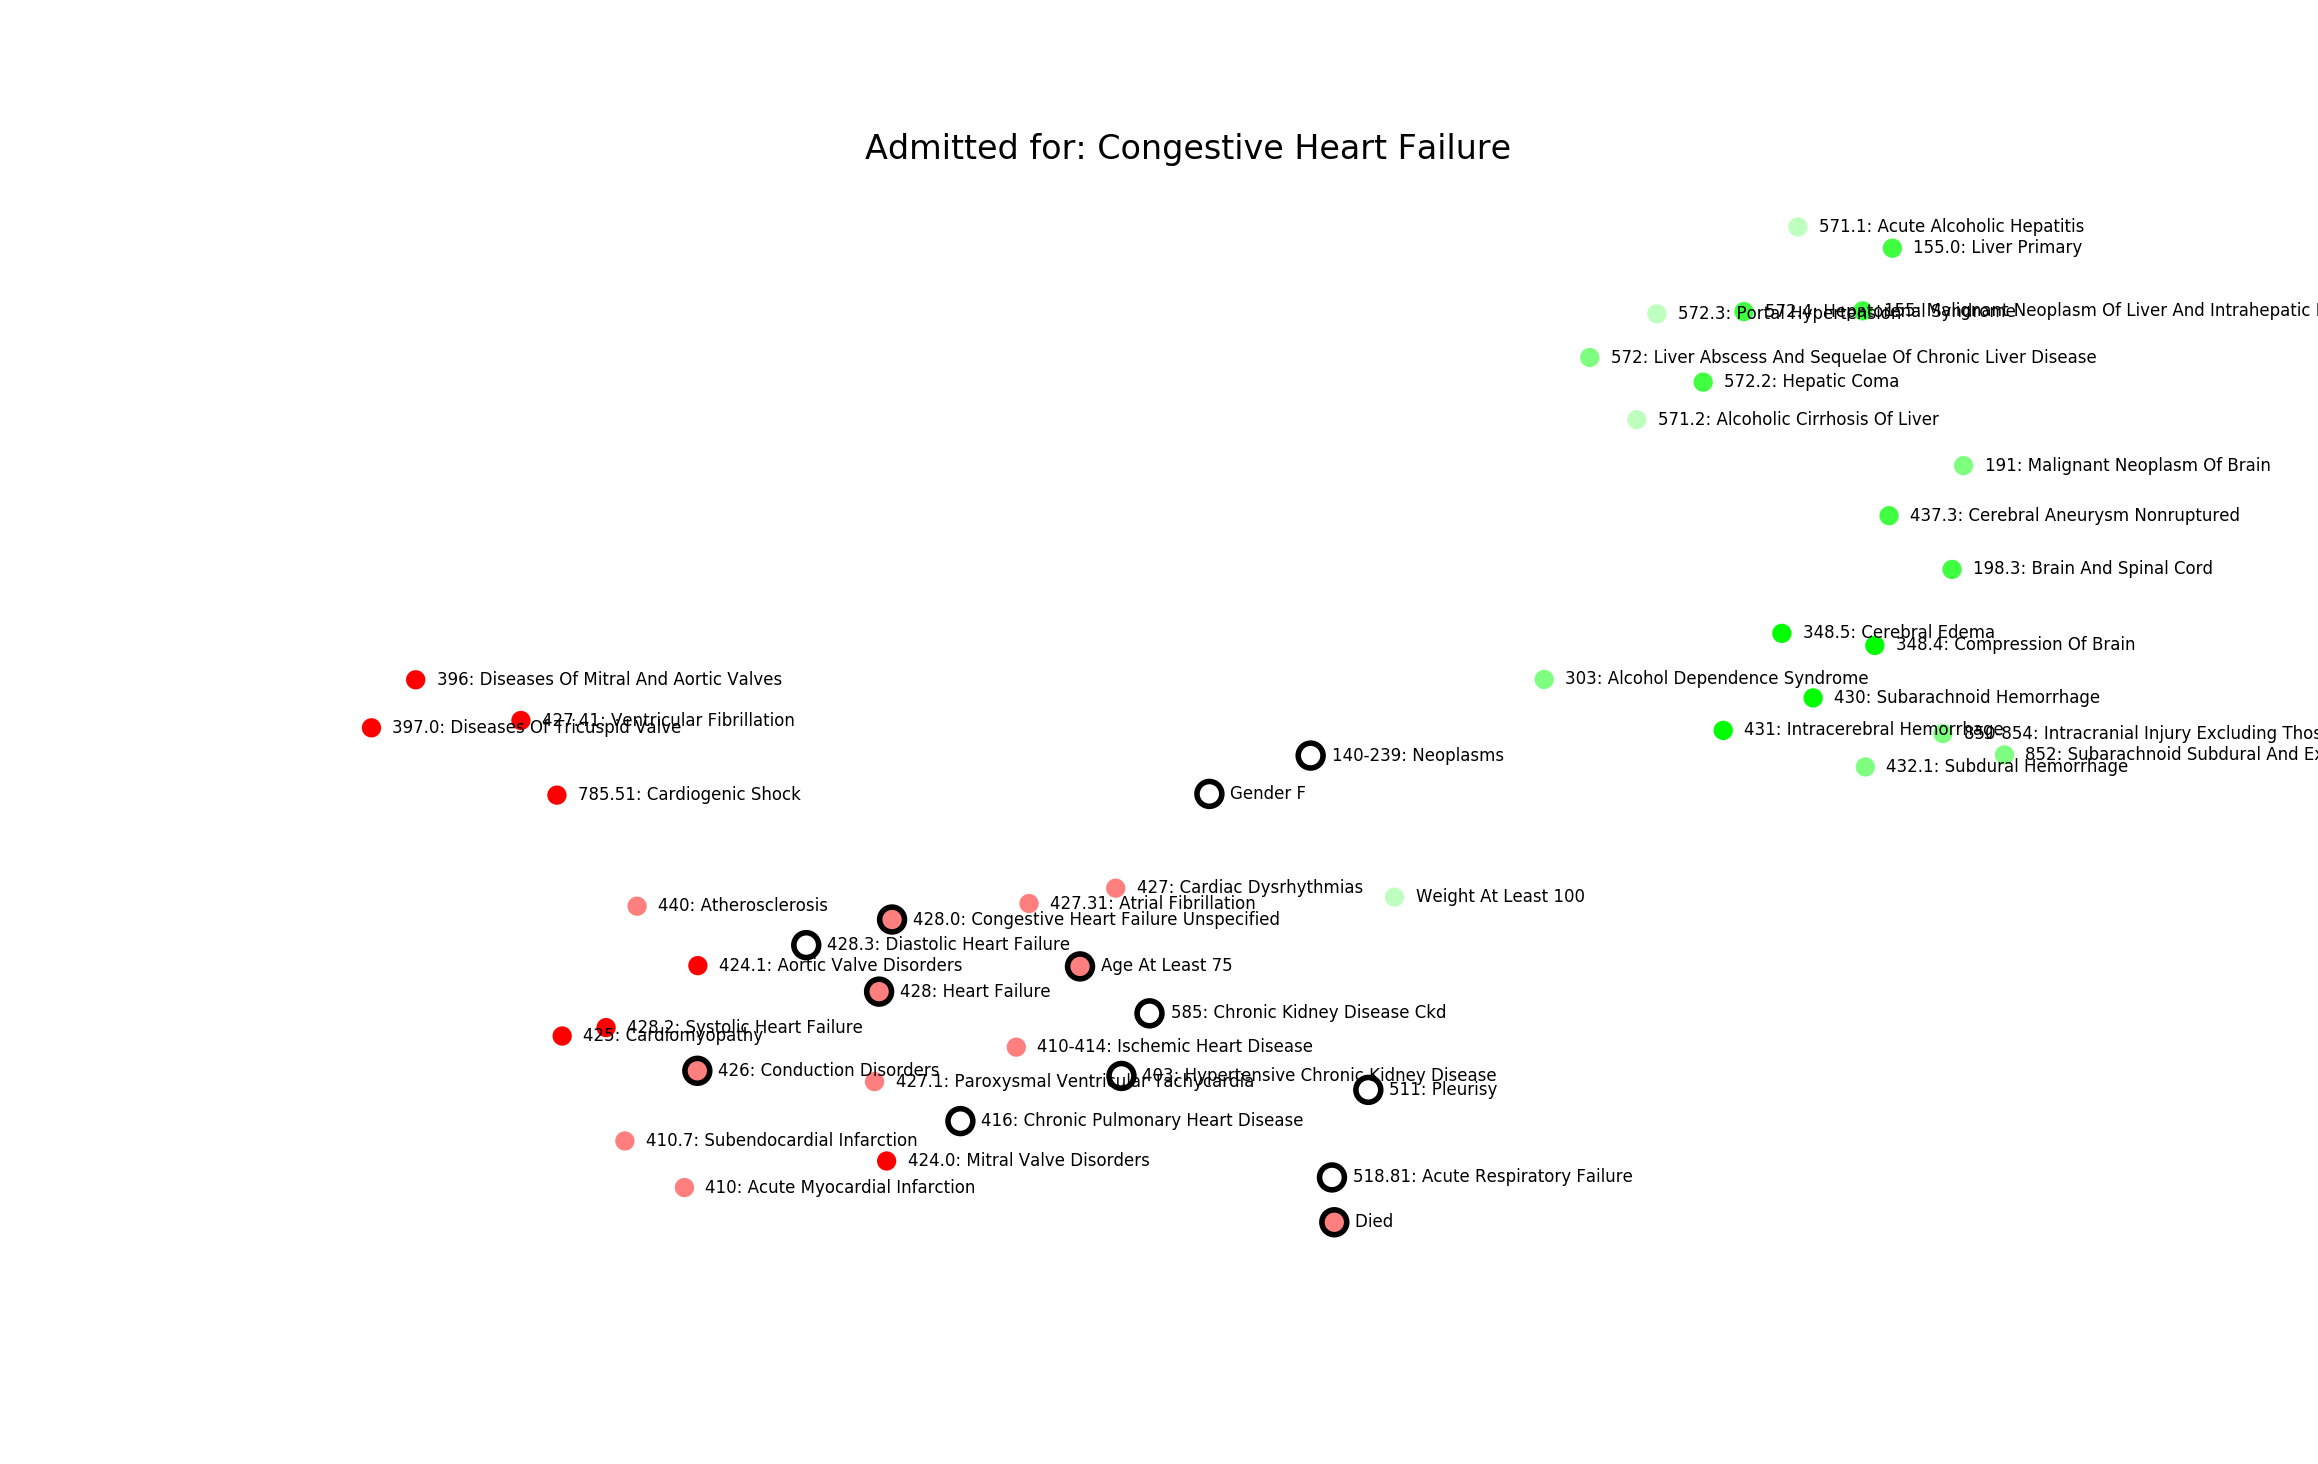
\includegraphics[width=\textwidth]{icu_map_chf}
    \caption{Semantic Inference Congestive Heart Failure}
    \vspace{12px}
    This patient was admitted for "Congestive Heart Failure".  The neural net predicted that they had low risk of liver and brain conditions (colored green).  It predicted high risk of heart conditions (colored red).  The patients was eventually diagnosed of conditions affecting the heart, and died (circled in black).
    \label{fig:icu_map_chf}
    \end{figure}
    
    % \begin{figure}
    % 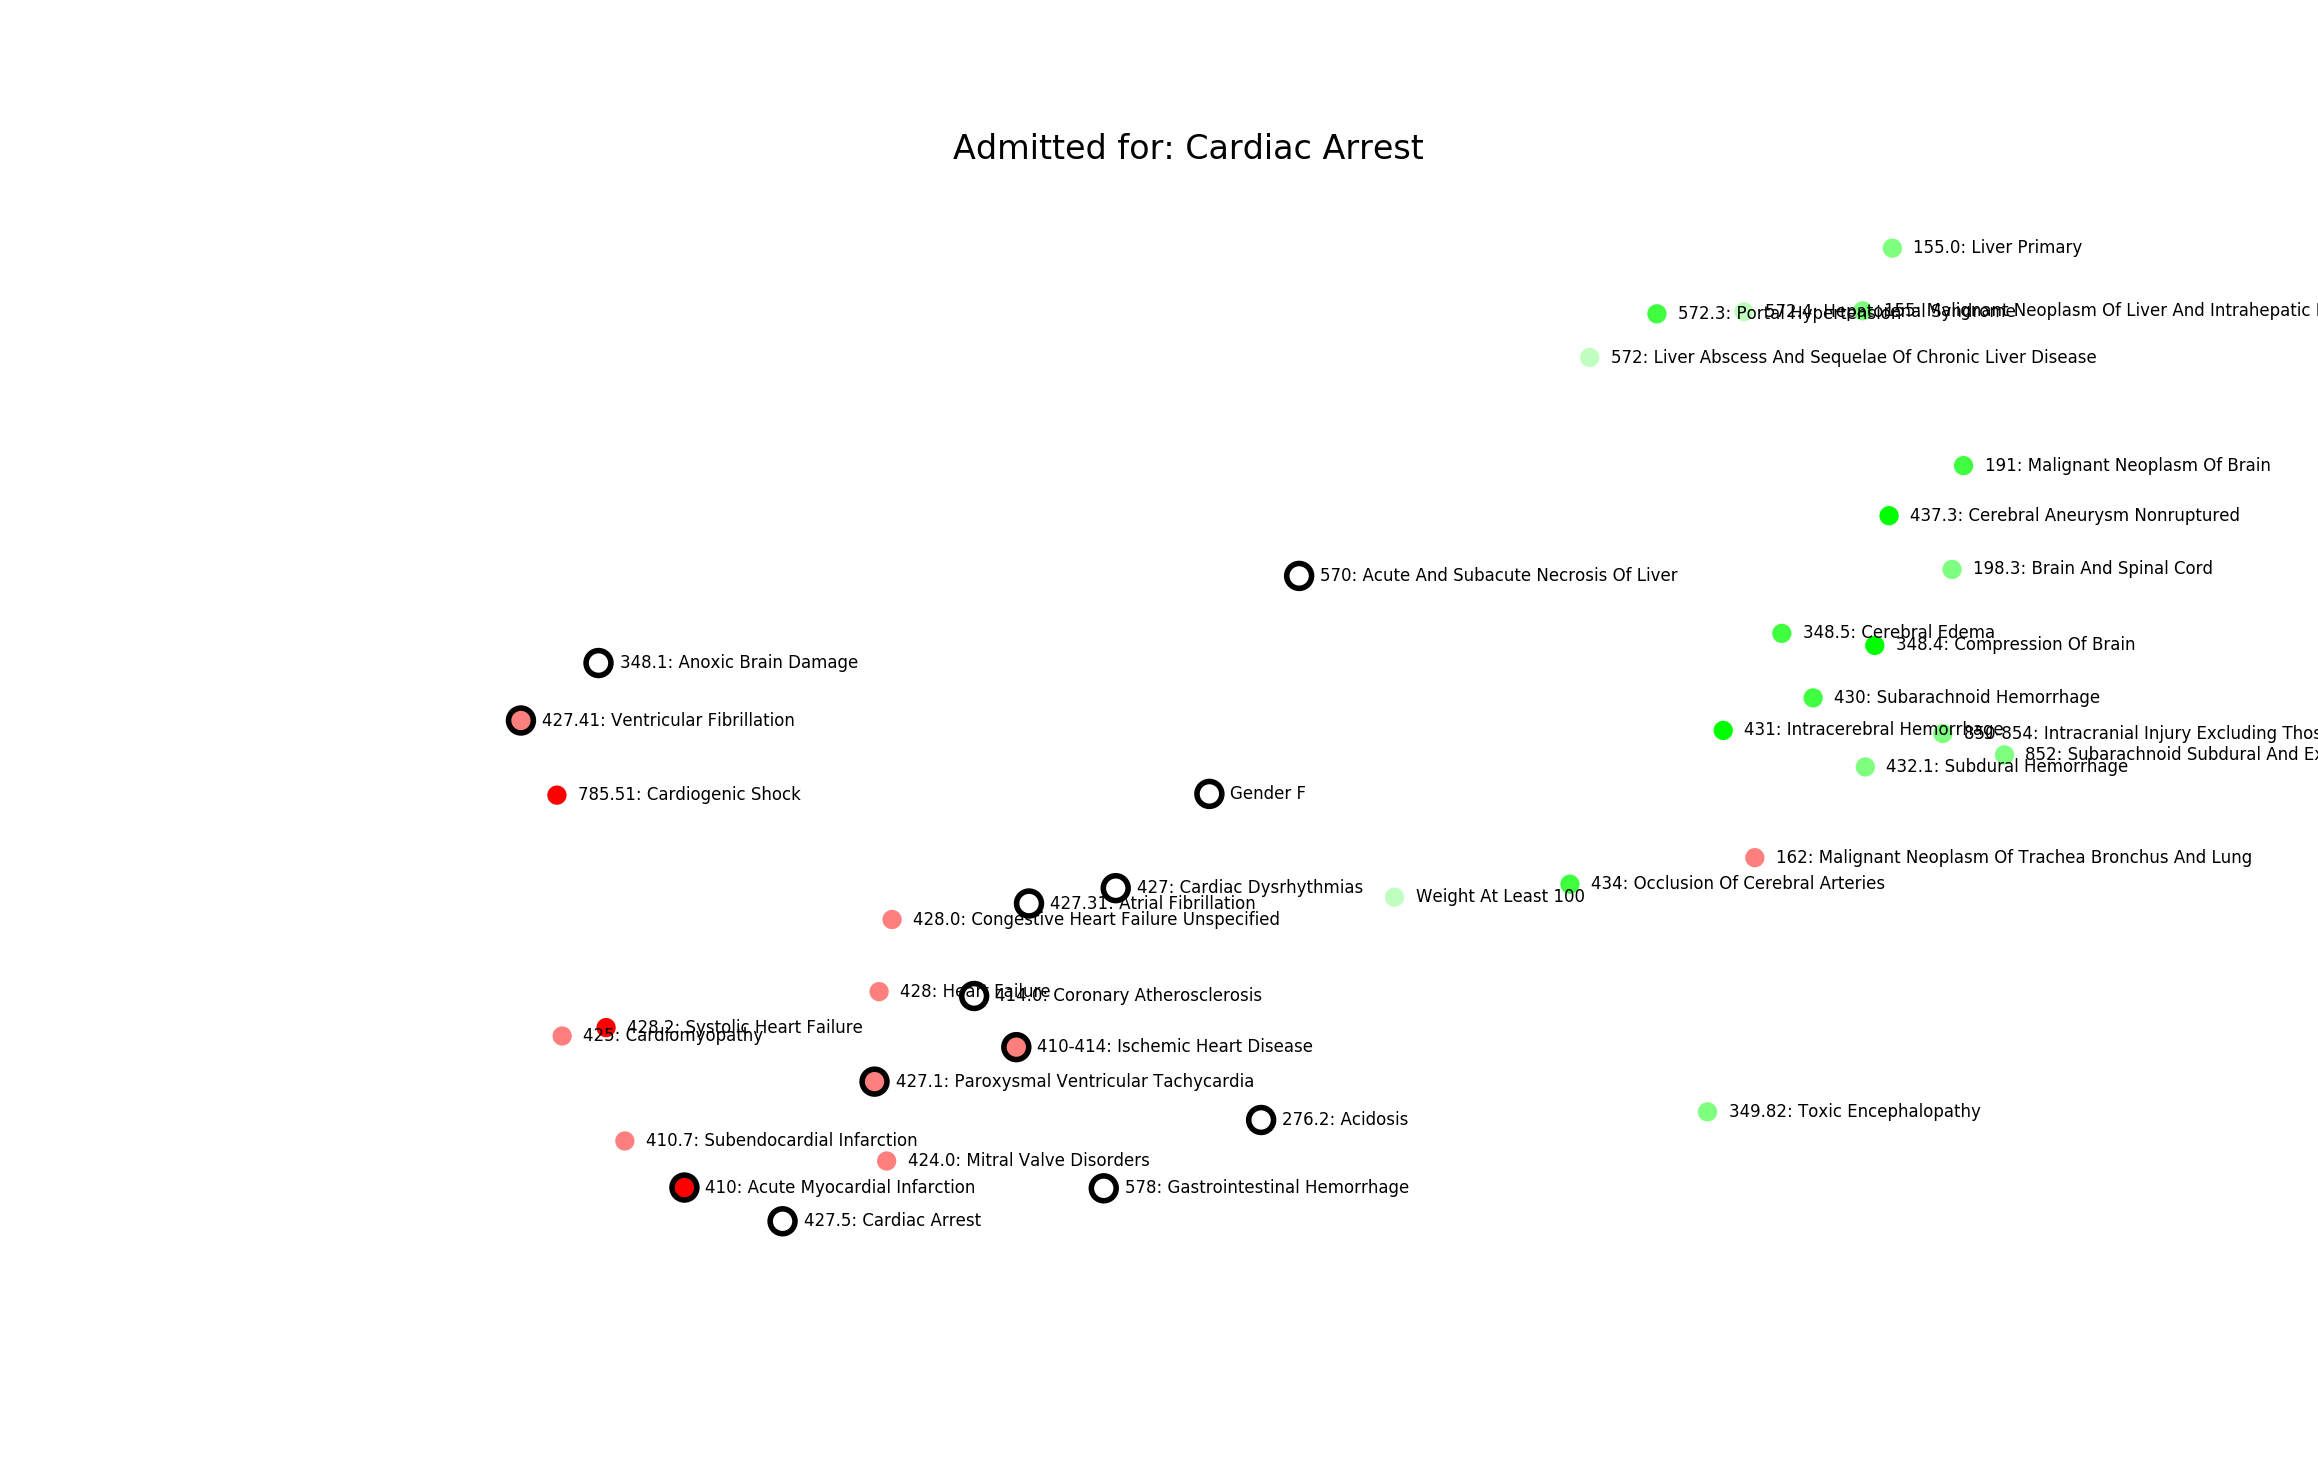
\includegraphics[width=\textwidth]{icu_map_cardarr}
    % \caption{Semantic Inference Cardiac Arrest}
    % \vspace{12px}
    % This patient was admitted for "Cardiac Arrest".  The neural net predicted that they had low risk of liver and brain conditions (colored green).  It predicted high risk of heart conditions (colored red).  The patients was eventually diagnosed of conditions affecting the heart among other things (circled in black).
    % \label{fig:icu_map_cardarr}
    % \end{figure}
    
    % \begin{figure}
    % 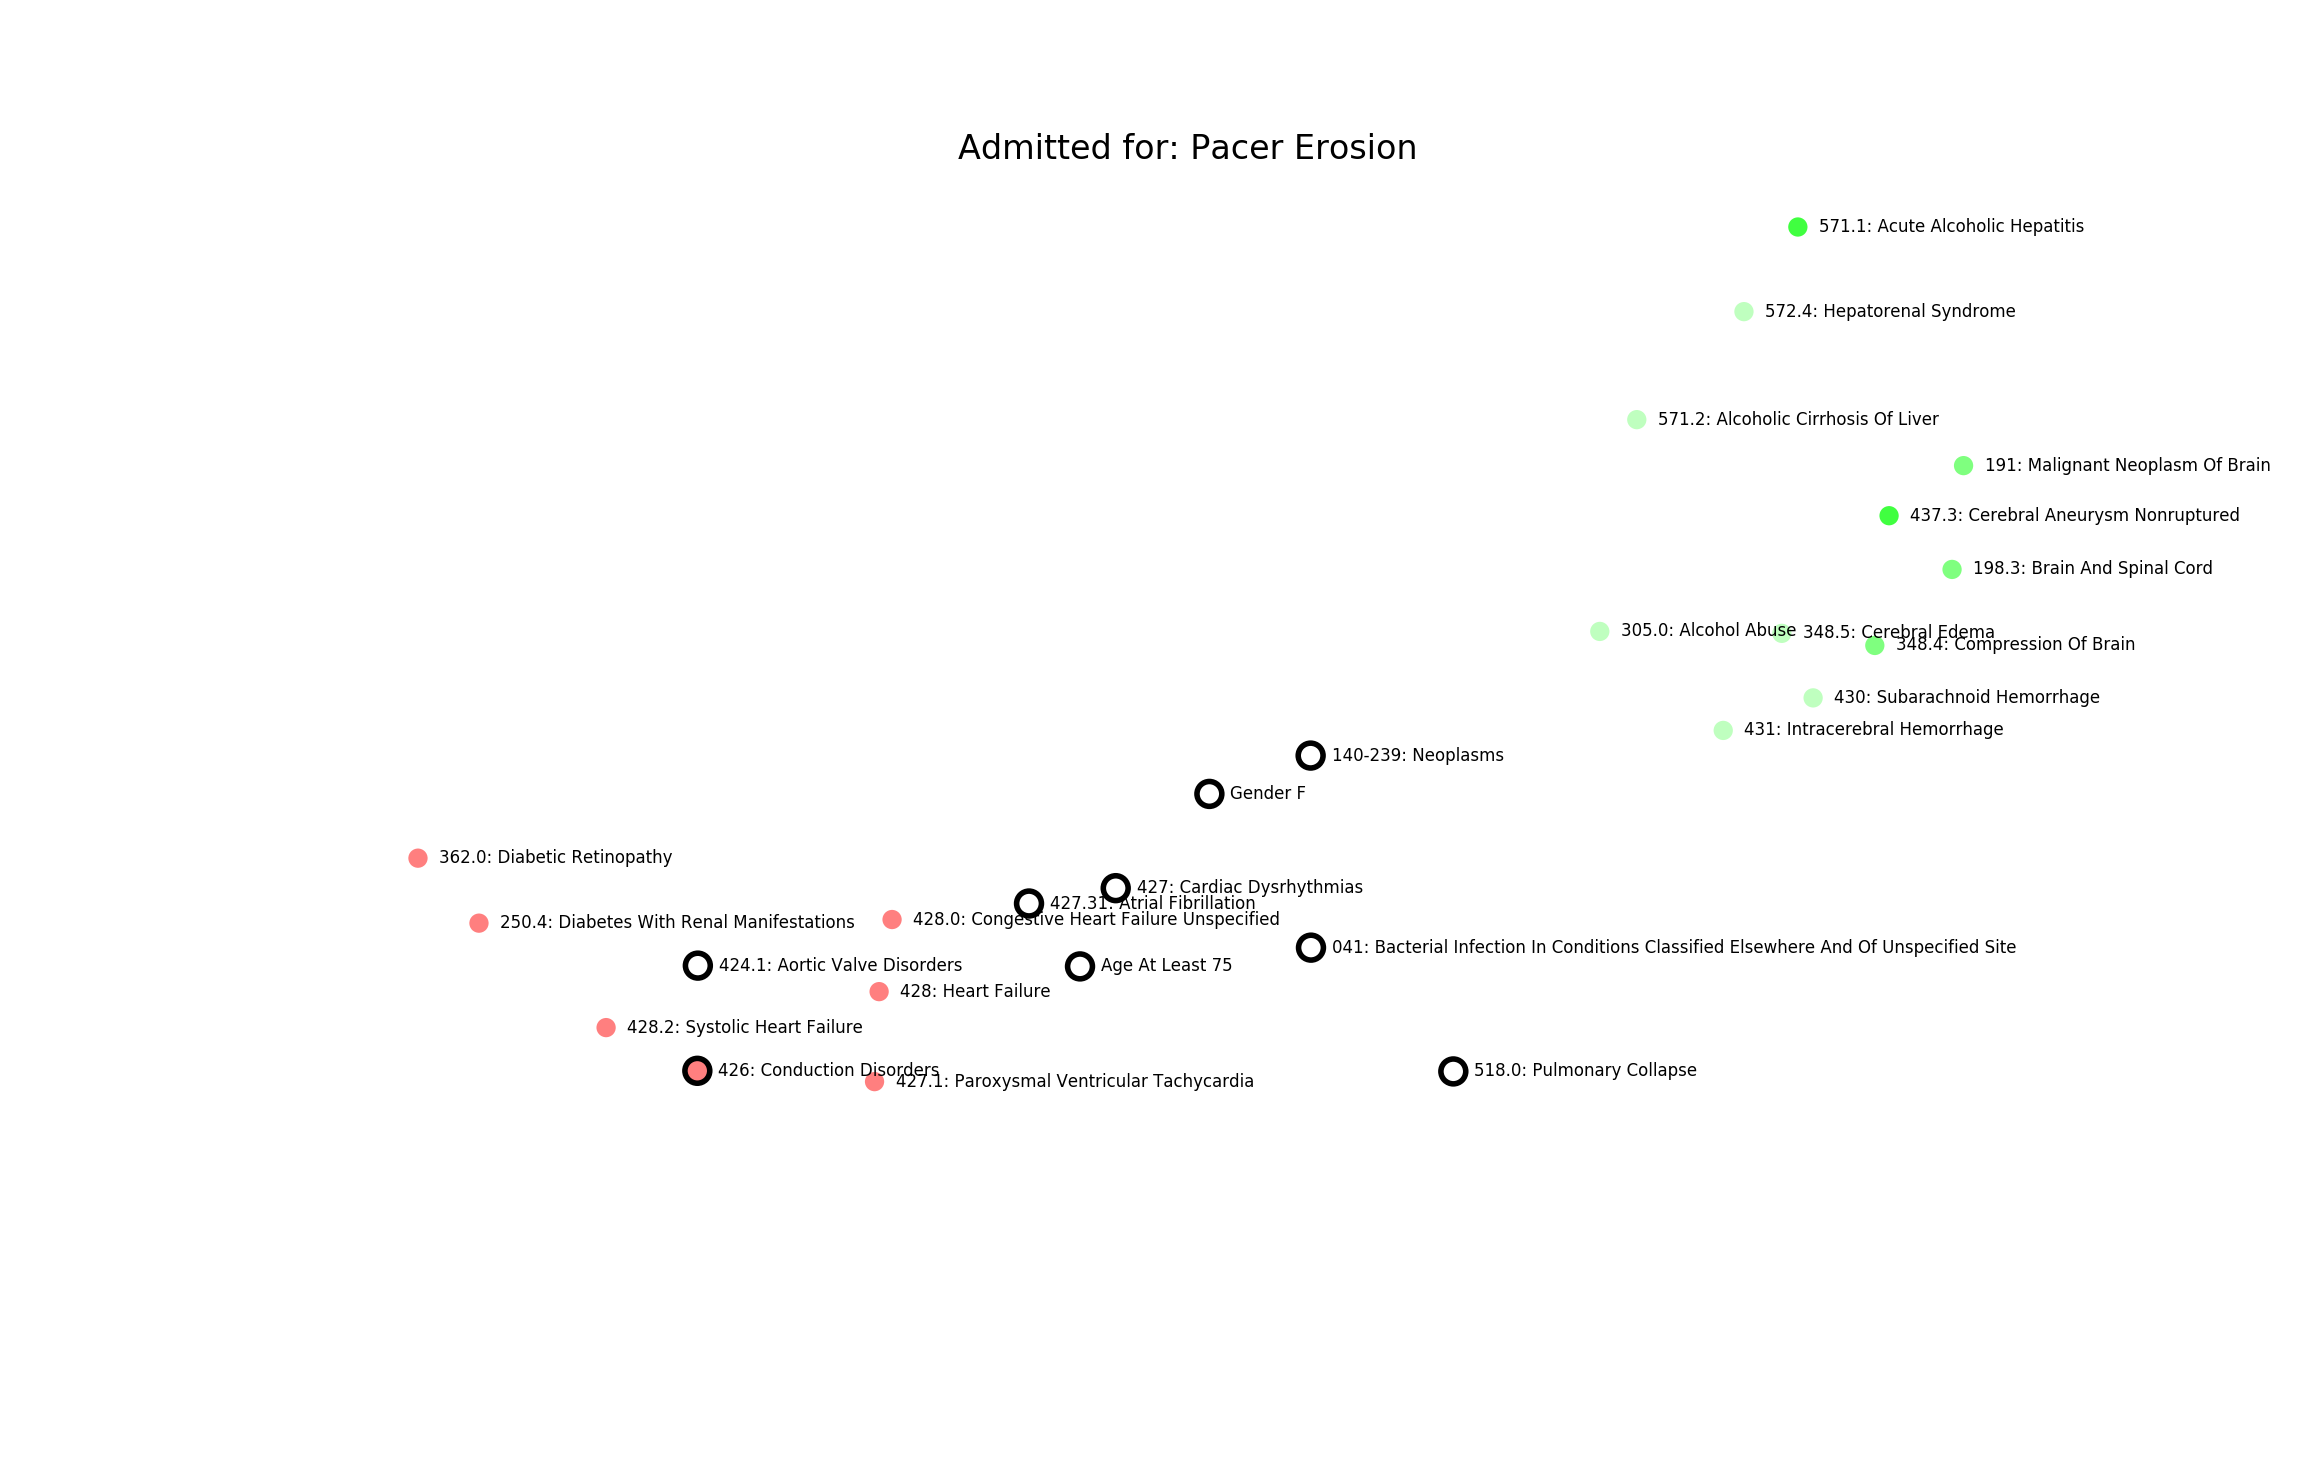
\includegraphics[width=\textwidth]{icu_map_pacer}
    % \caption{Semantic Inference Pacer Erosion}
    % \vspace{12px}
    % This patient was admitted for "Pacer Erosion".  The neural net predicted that they had low risk of liver and brain conditions (colored green).  It predicted high risk of heart conditions (colored red).  The patients was eventually diagnosed of conditions affecting the heart (circled in black).
    % \label{fig:icu_map_pacer}
    % \end{figure}
    
    % \begin{figure}
    % 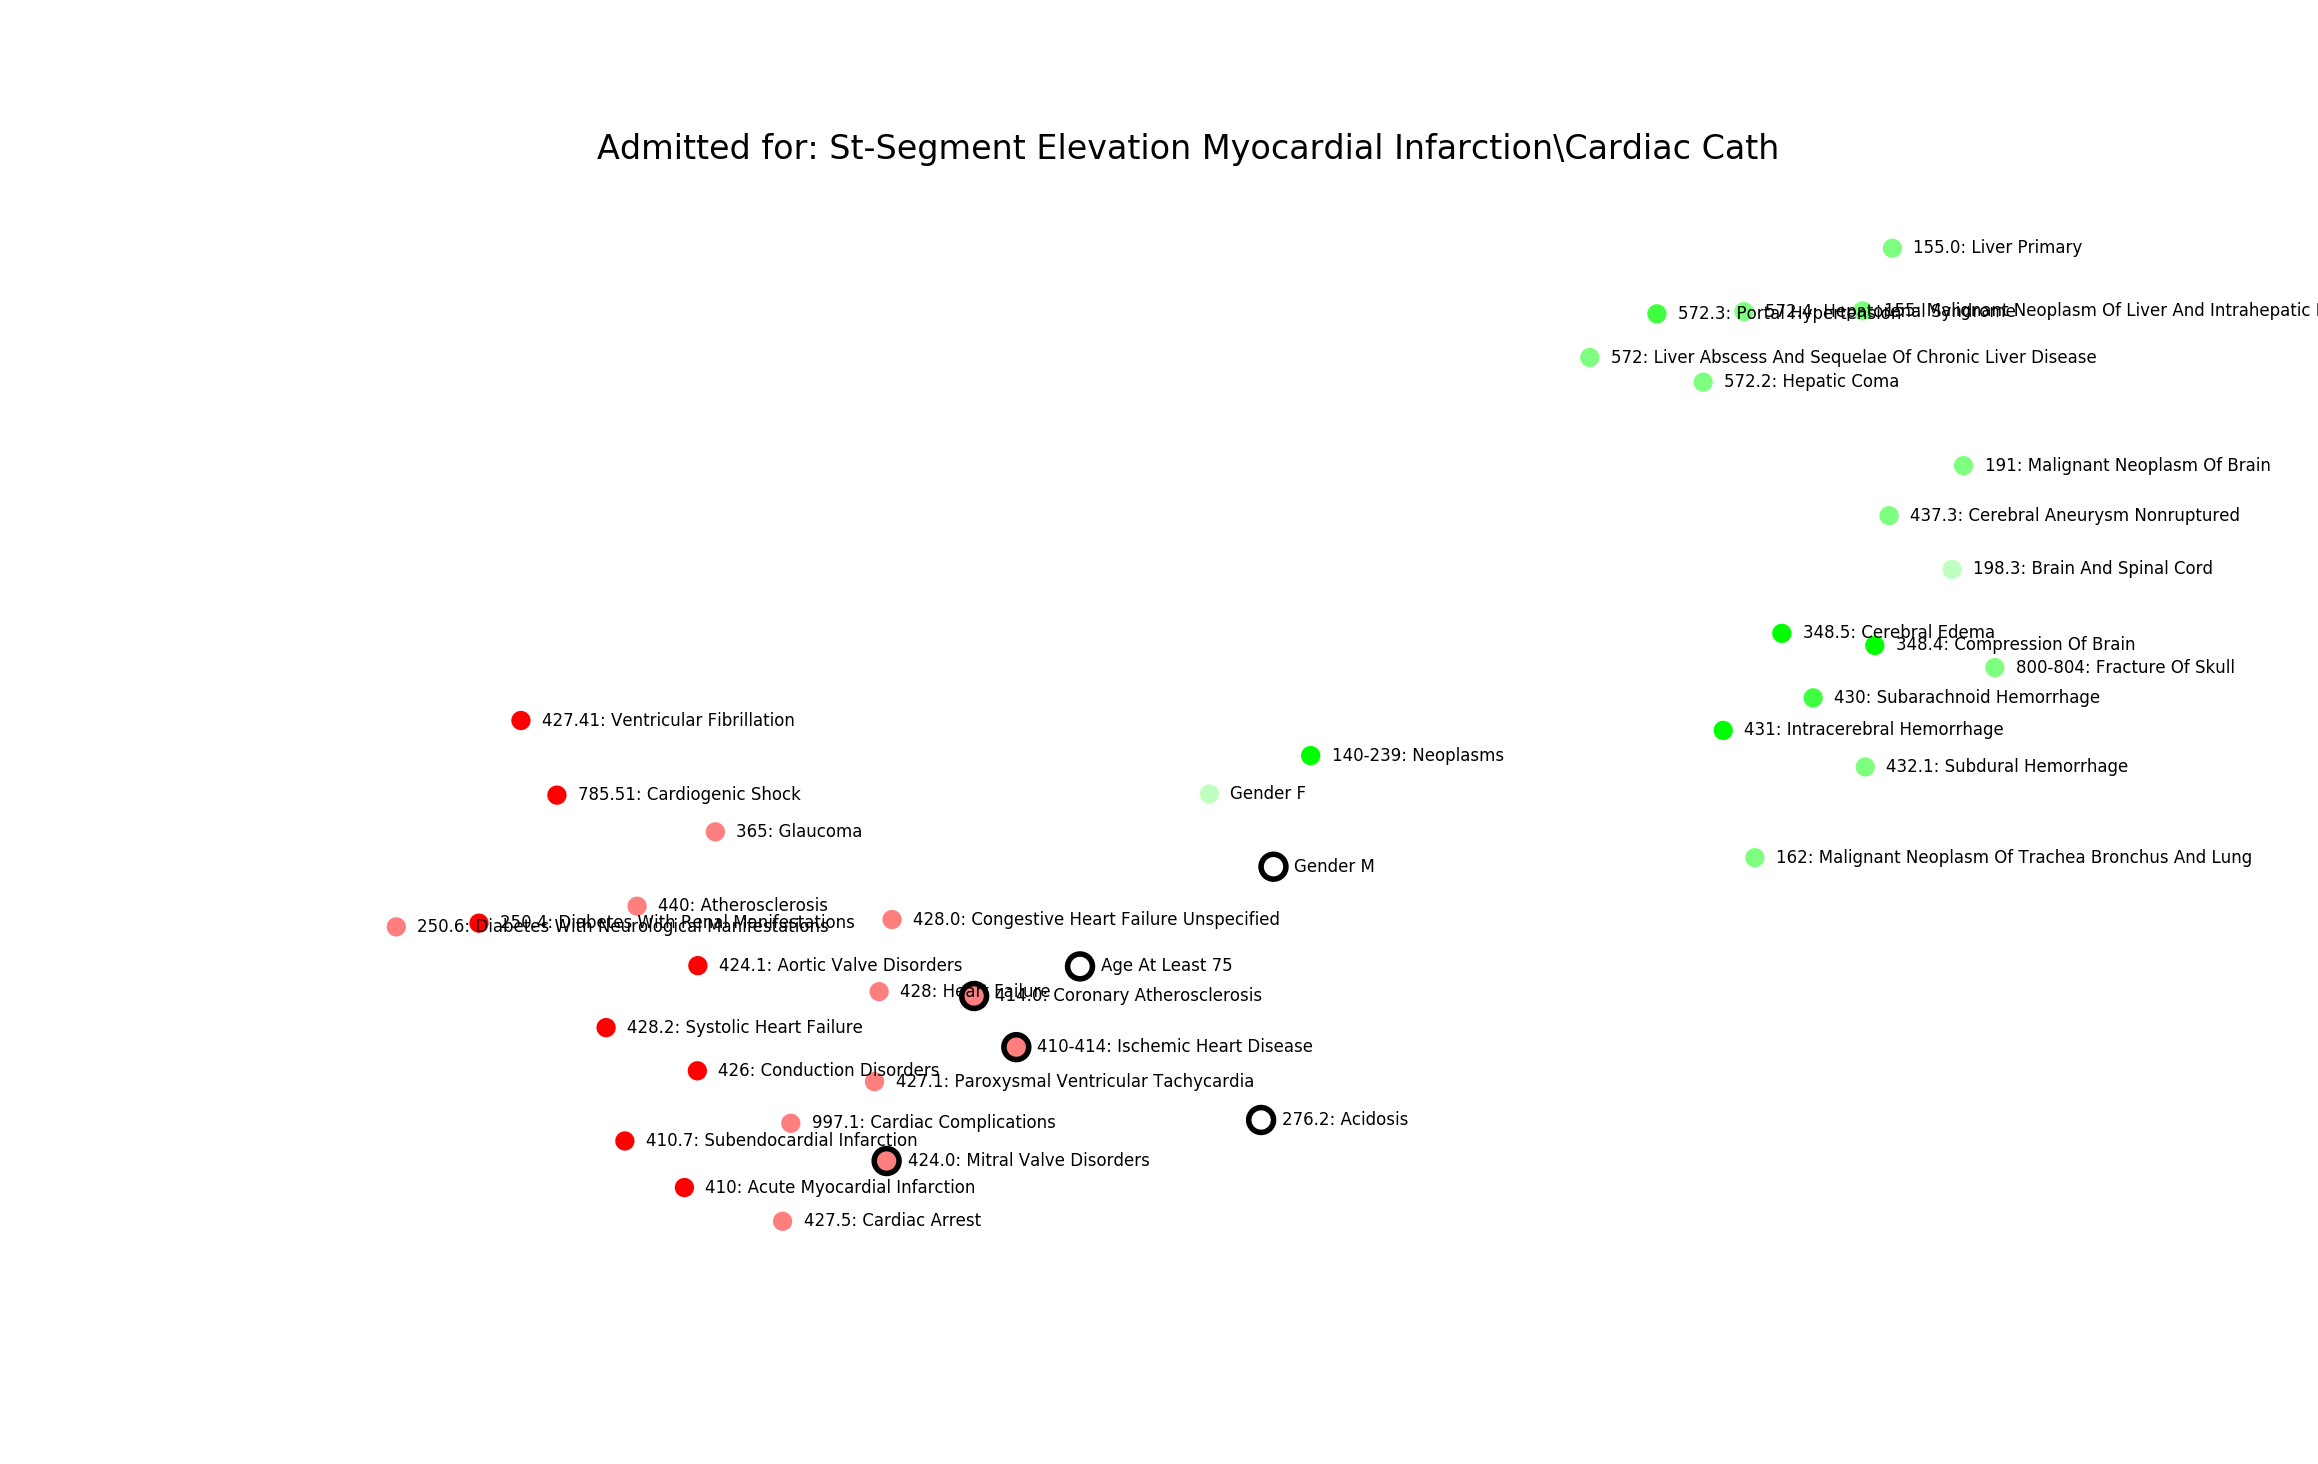
\includegraphics[width=\textwidth]{icu_map_stseg}
    % \caption{Semantic Inference ST Elevation}
    % \vspace{12px}
    % This patient was admitted for "St-Segment Elevation Myocardial Infarction/Cardiac Cath".  The neural net predicted that they had low risk of liver and brain conditions (colored green).  It predicted high risk of heart conditions (colored red).  The patients was eventually diagnosed of conditions affecting the heart (circled in black).
    % \label{fig:icu_map_stseg}
    % \end{figure}
    
    % \begin{figure}
    % 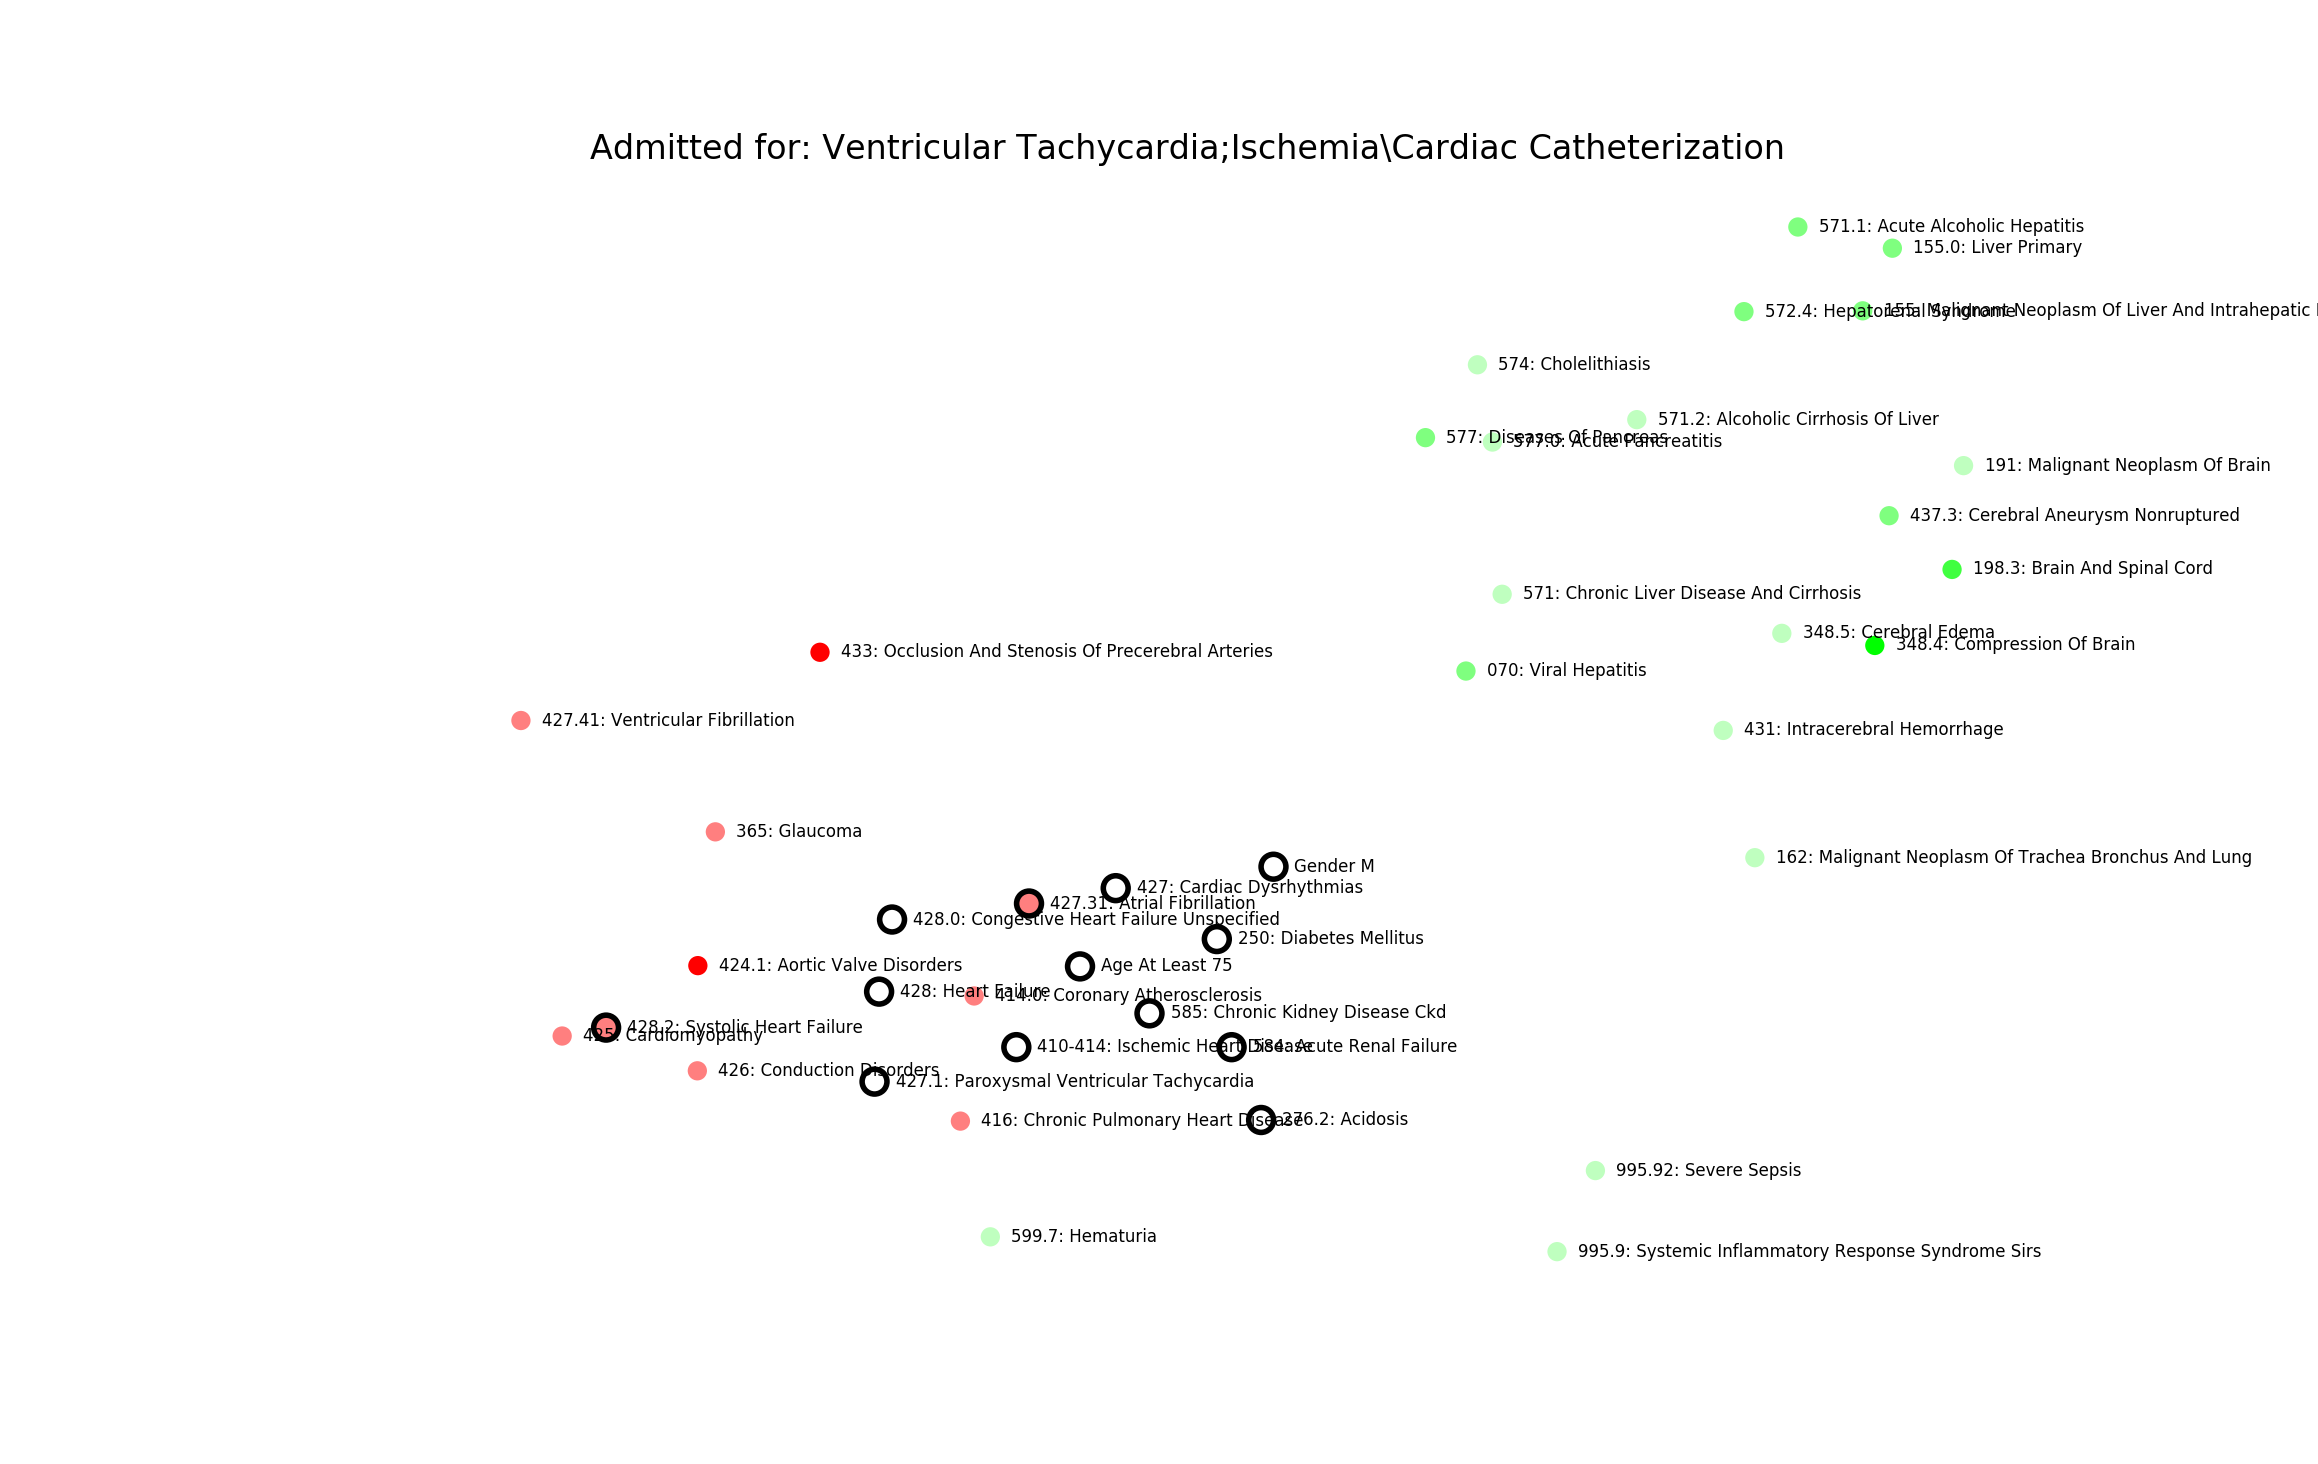
\includegraphics[width=\textwidth]{icu_map_ventach}
    % \caption{Semantic Inference Ventricular Tachycardia}
    % \vspace{12px}
    % This patient was admitted for ventricular tachycardia.  The neural net predicted that they had low risk of liver and brain conditions (colored green).  It predicted high risk of heart conditions (colored red).  The patients was eventually diagnosed of conditions affecting the heart (circled in black).
    % \label{fig:icu_map_ventach}
    % \end{figure}
    
    \begin{figure}
    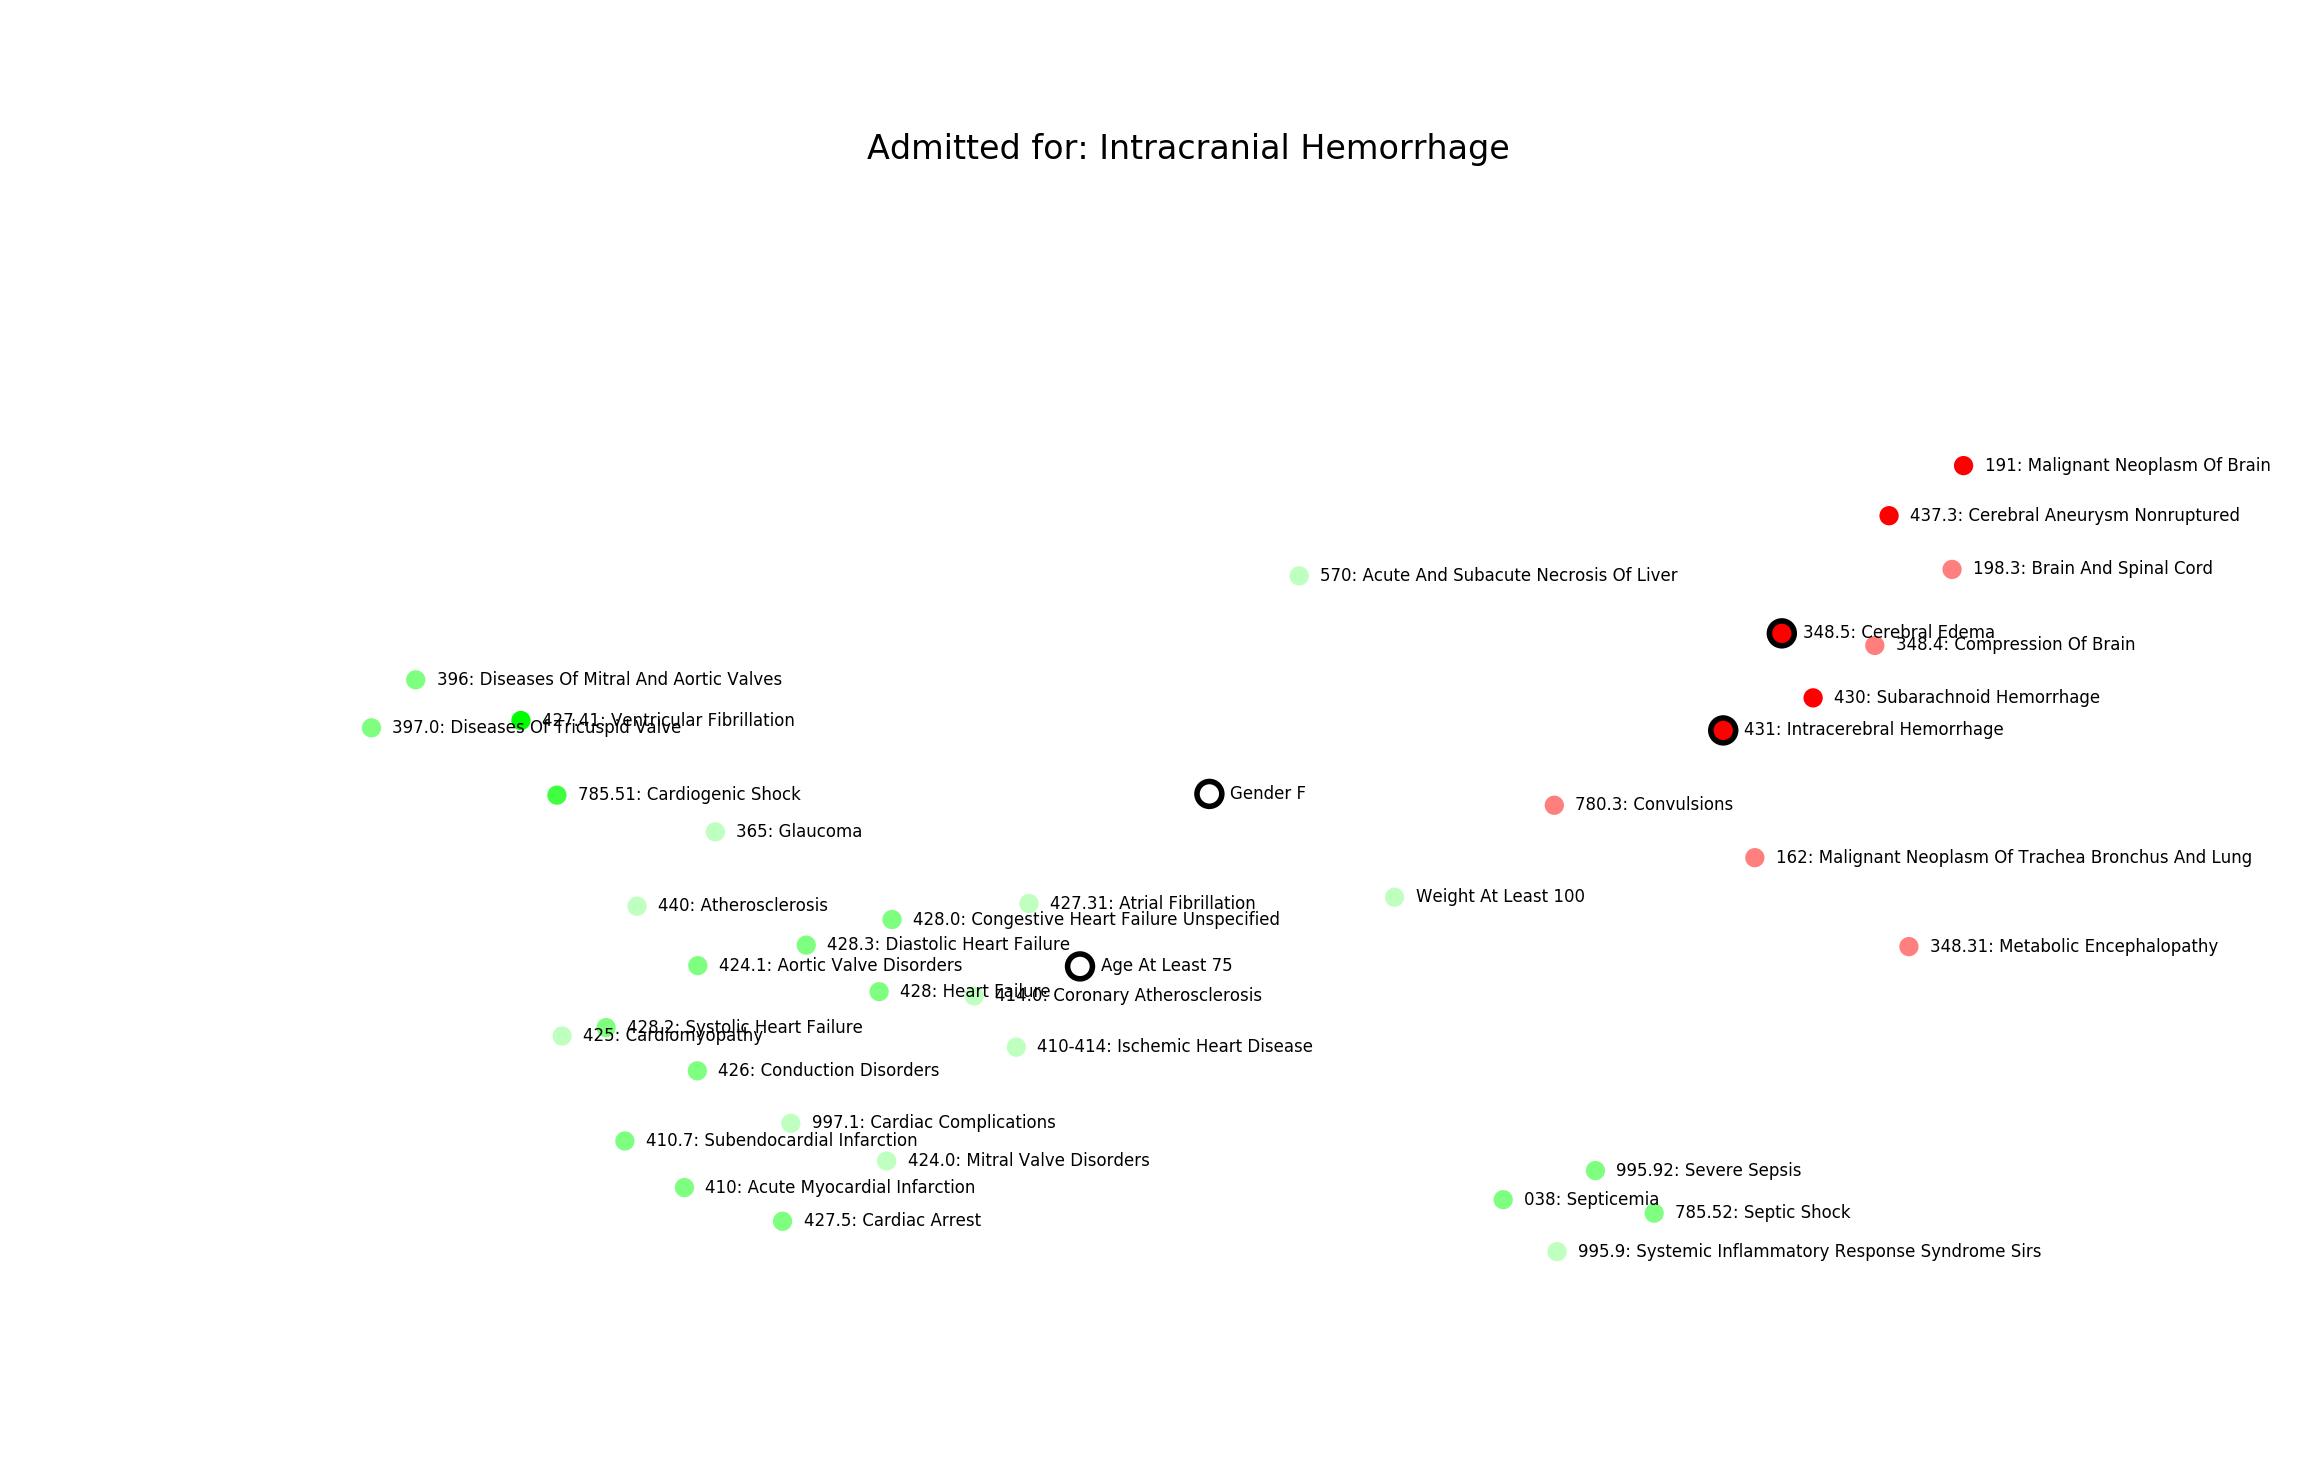
\includegraphics[width=\textwidth]{icu_map_brain}
    \caption{Semantic Inference Intracranial Hemorrhage}
    \vspace{12px}
    This patient was admitted for "Intracranial Hemorrhage".  The neural net predicted that they had low risk of heart conditions and septic conditions (colored green).  It predicted high risk of brain conditions (colored red).  The patients was eventually diagnosed with cerebral edema and intracerebral hemorrhage (circled in black).
    \label{fig:icu_map_brain}
    \end{figure}
    
    \begin{figure}
    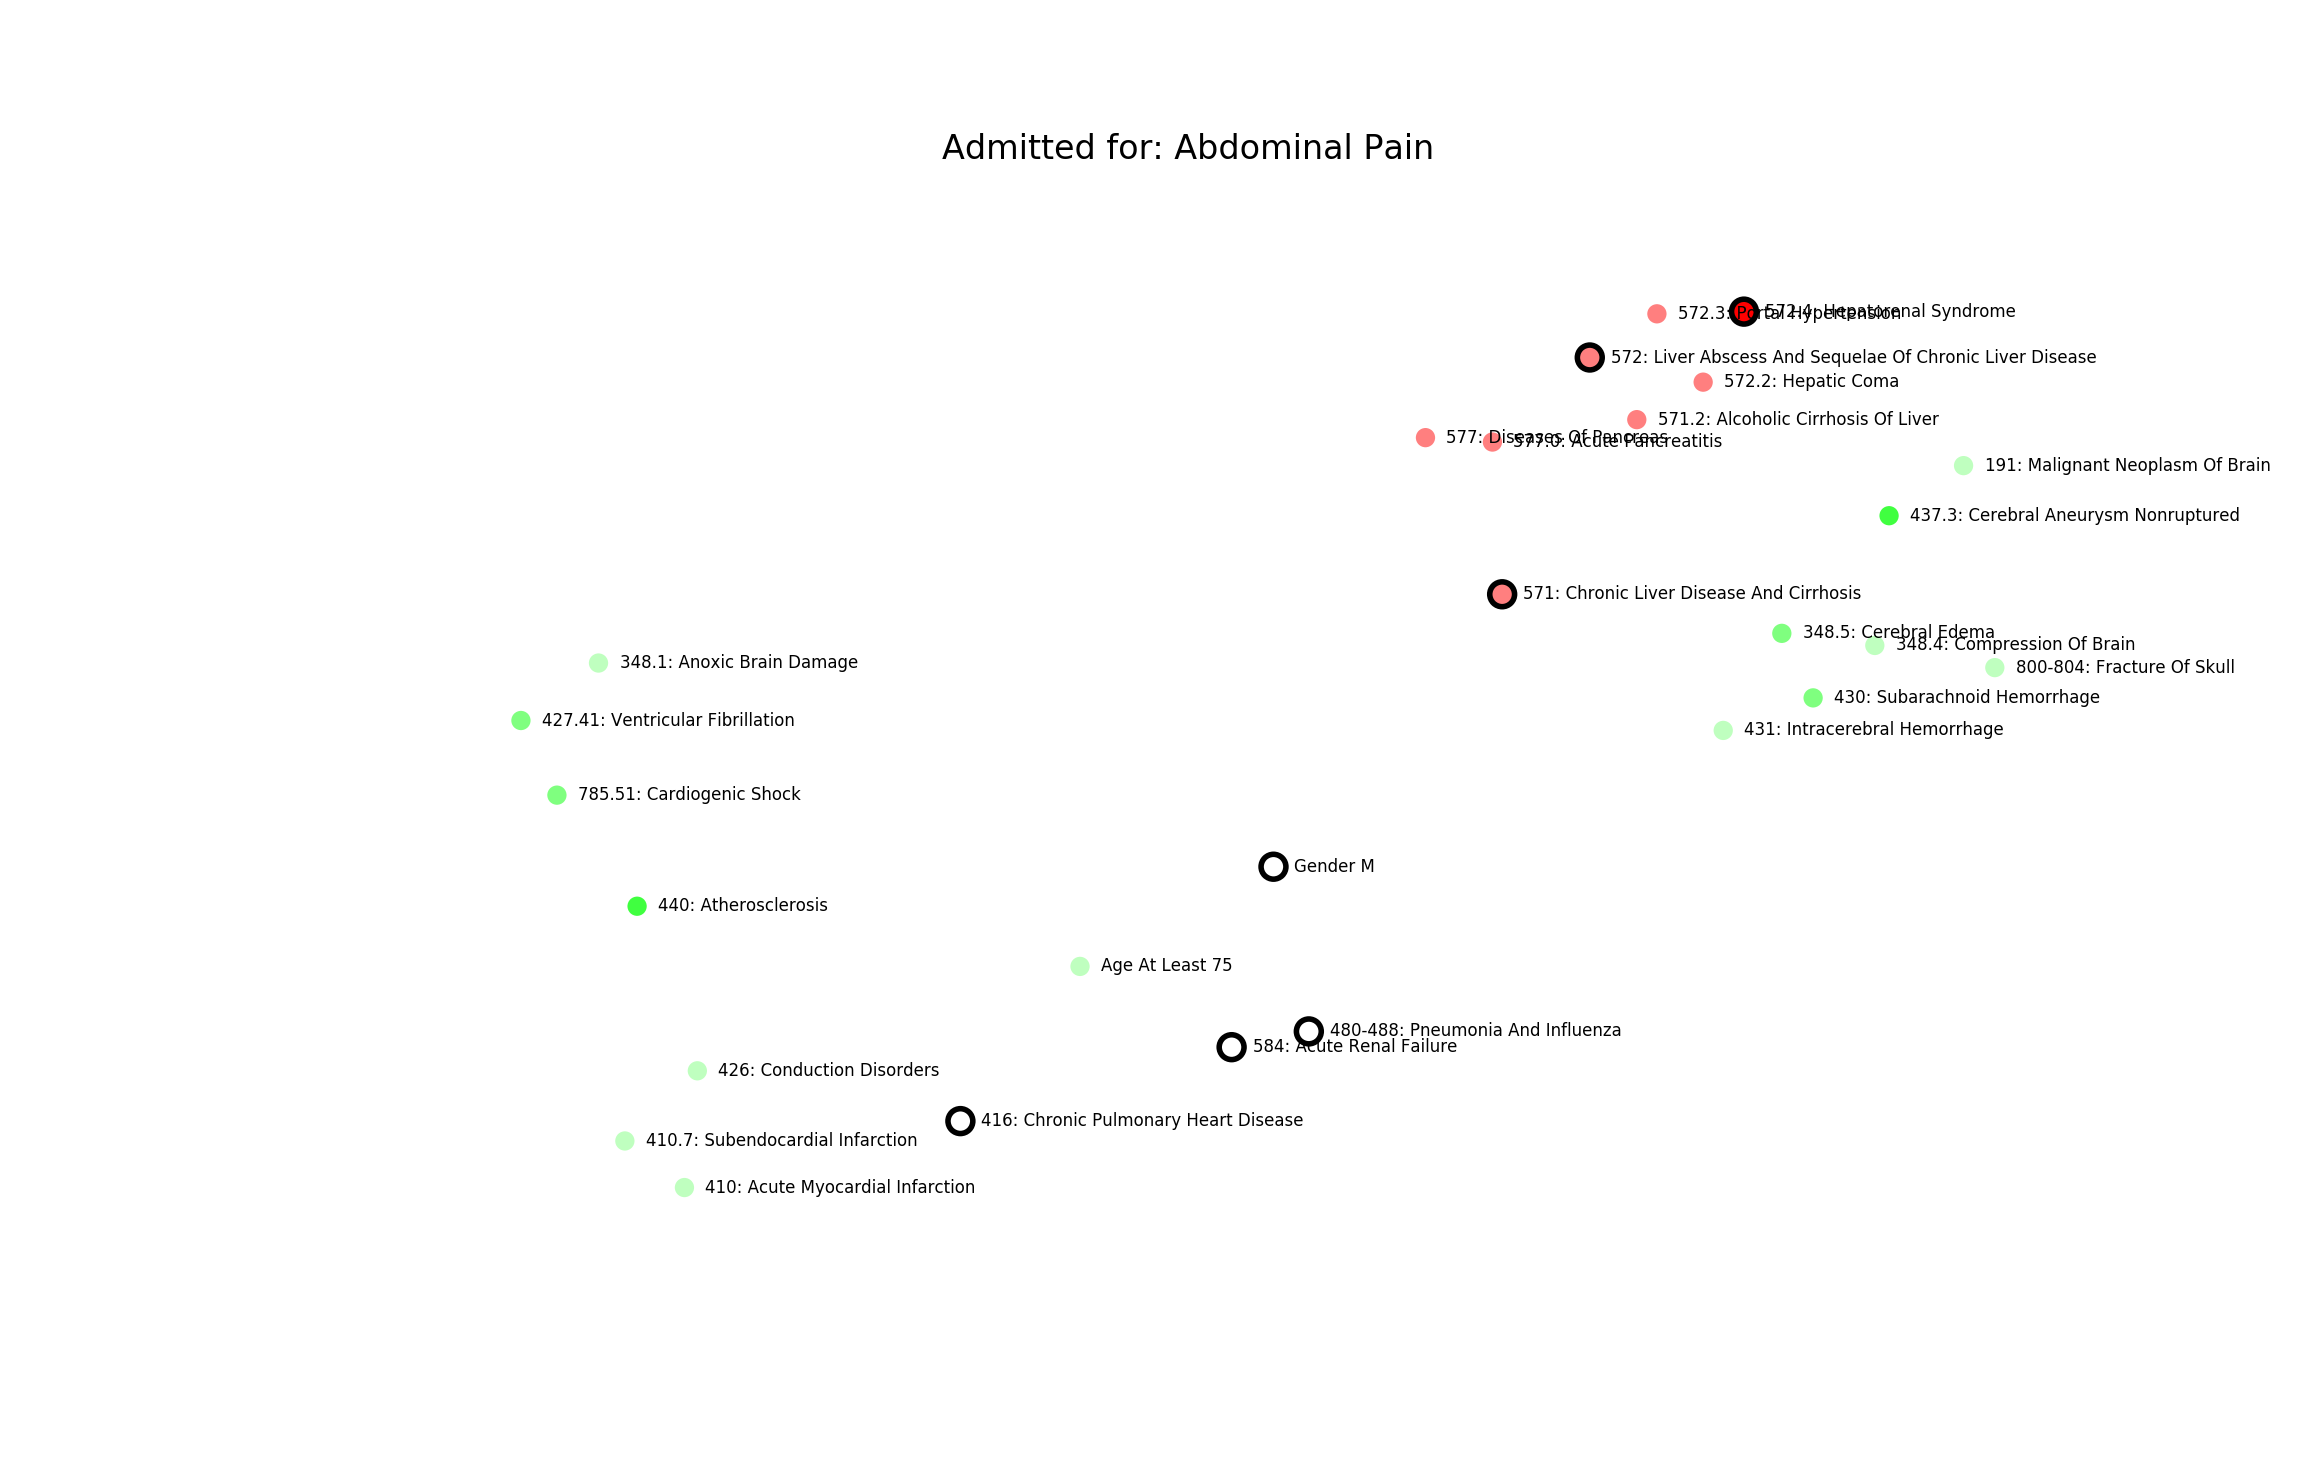
\includegraphics[width=\textwidth]{icu_map_liver}
    \caption{Semantic Inference Abdominal Pain}
    \vspace{12px}
    This patient was admitted for "Abdominal Pain".  The neural net predicted that they had low risk of brain and heart conditions (colored green).  It predicted high risk of liver conditions (colored red).  The patients was eventually diagnosed with chronic liver cirrhosis and a liver abscess among other things (circled in black).
    \label{fig:icu_map_liver}
    \end{figure}
}